%------------------------------------%
%			Inicio Preámbulo
%------------------------------------%
\documentclass[12pt,spanish]{thesis}
% Mayor compatibilidad y preferencia personal
%\usepackage[latin1]{inputenc}
\usepackage[utf8]{inputenc}
\usepackage[spanish]{babel}
\usepackage{amsmath}

% Interlineado
\usepackage{setspace}
\setstretch{1.5}

% Paquetes
\usepackage{textcomp}
\usepackage{times}
\usepackage{amssymb}
\usepackage{float}
\usepackage{color}
\usepackage{graphicx}
\usepackage{eso-pic}
\usepackage{multicol}
\usepackage{enumerate}
\usepackage{url}
\usepackage{soul}
\usepackage{fancyhdr}
\usepackage{lscape}
\usepackage{pdfpages}
\usepackage{hyperref}
\usepackage{listings}


% Márgenes
\usepackage[top=3cm,bottom=3cm,left=4.2cm,right=3cm]{geometry}
\pagestyle{empty} 
\frenchspacing
\fancyhead[L]{}
\fancyhead[C]{}
\fancyhead[R]{}
\fancyfoot[R]{\thepage}
\fancyfoot[C]{}

%------------------------------------%
%			Fin Preámbulo
%------------------------------------%


\begin{document}
\thispagestyle{empty}

\begin{center}
%\linespread{1.15}
\renewcommand{\baselinestretch}{1.15}
\textbf{\large{UNIVERSIDAD TÉCNICA FEDERICO SANTA MARÍA\\}
\normalsize{DEPARTAMENTO DE ELECTRÓNICA\\VALPARAÍSO - CHILE\\}}

\vspace{0.5cm}
\begin{figure}[H]
\centering
  
\includegraphics[width=5.85cm]{figuras/usmLogo.png}
\end{figure}
\vspace{0.5cm}

%\linespread{1}
\renewcommand{\baselinestretch}{1}
\hangindent=0cm
\textbf{\Large ``Sistema de monitoreo de pacientes cardíacos en tiempo real, utilizando una aplicación Android con tecnologías Bluetooth y WebSocket''\\}
\vspace{3cm}
\hangindent=0cm\large \textbf{Patricio Rodríguez Gatica}\\
\vspace{0.5cm}
\hangindent=0cm\normalsize \textbf{MEMORIA DE TITULACIÓN PARA OPTAR AL TÍTULO DE INGENIERO CIVIL TELEMÁTICO}\\
\vspace{1cm}
\hangindent=0cm\normalsize \textbf{PROFESOR GUIA: \hspace{2cm} Marcos Zúñiga B.}\\
\vspace{0.5cm}
\hangindent=0cm\normalsize \textbf{PROFESOR CORREFERENTE: \hspace{2cm} Francisco Cabezas B.}\\
\vspace{0.5cm}
\hangindent=0cm\normalsize \textbf{PROFESOR CORREFERENTE: \hspace{2cm} Daniel Erraz L.}\\

\end{center}

\thispagestyle{empty}
\newpage
\pagestyle{fancy}
\renewcommand\headrulewidth{0pt}
\renewcommand{\listfigurename}{Índice de figuras}
\renewcommand{\listtablename}{Índice de tablas}

%Numeros romanos al pie de pagina, secciones sin numero.
\pagenumbering{roman}

\section*{Agradecimientos}

Agradecer es un paso fundamental en todo desarrollo humano, puesto que es de las pocas oportunidades de reflexionar sobre quienes estuvieron y están a nuestro lado en alguna etapa de nuestra vida. Me gustaría destacar que aun cuando agradecer es una vista al pasado, no existe tiempo inconexo en el corazón y los llevo siempre conmigo.

Quiero agradecer a mi familia, mi pareja, amigos, compañeros, profesores y toda persona con quien he tenido contacto en esta etapa universitaria, todos me han formado y son parte de este trabajo de una o de otra manera.

Le dedico este trabajo a quienes siempre creyeron en mí y a quienes aun lo hacen. Porque incluso teniendo un núcleo familiar distinto, el amor y la comprensión siempre estuvieron conmigo: A mi padre Omar Bernales Vega, a mis madres Toya y Mónica Gatica y mis hermanas Bárbara, Elein y Maka. Son mi orgullo y mi ejemplo a seguir.

Por último y no por ello menos importante, a la persona que soportó mis rabietas y jornadas de estrés, quien aun me acompaña y ama de forma extraordinaria, mi Valeria.

\newpage

\section*{Resumen}

El presente documento relatará la resolución de un problema real y actual en Chile, a partir de un desafío propuesto en el contexto de las Memorias Multidisciplinarias.\par
El desafío consiste en el desarrollo de un sistema con la capacidad de monitorear pacientes de forma remota, de bajo costo y con las limitantes geográficas propias de nuestro país, teniendo en mente su aplicación a nivel público del Sistema de Salud. Para esto, se analizaron las distintas opciones existentes en el mercado y se desarrolló una solución a nivel de prototipo funcional que cumpliese con las restricciones ya mencionadas.\par
Por ser un desafío resuelto de forma multidisciplinaria es importante destacar que el desarrollo en este documento estará enfocado al área informática y de telecomunicaciones asociada a la adquisición, procesamiento, almacenamiento y envío de datos.\par
El resto del equipo final está compuesto por: Sebastián Castillo actual Ingeniero en Diseño de Productos y Felipe Cordero actual Ingeniero Civil Electrónico, ambos de la misma casa de estudios UTFSM. Ambas memorias complementan la actual en el ámbito correspondiente a sus carreras, pero lógicamente compartiendo su núcleo como proyecto conjunto.
\newpage

%\section*{Abstract}

%\newpage

\section*{Glosario}

\begin{tabular}{lcp{10.5cm}}
RF &:& Radio Frecuencia\\
	
Wi-Fi &:& Proviene del termino Wireless Fidelity. Corresponde a la norma IEEE 802.11
que define los estándares de conectividad inalámbrica para transmisión de datos entre dispositivos.\\


Esquemático &:& Es una representación pictórica de un circuito electrónico. Muestra las diferentes componentes del circuito de manera simple y las conexiones de alimentación y señales entre distintos dispositivos.\\
PCB &:& Printed Circuit Board, El circuito impreso se utiliza para conectar eléctricamente a través de las pistas conductoras, y sostener mecánicamente, por medio de la base, un conjunto de componentes electrónicos.\\
Hardware &:& Partes físicas tangibles de un sistema informático.\\
Software &:& Aplicaciones o programas que funcionan en un sistema informático.\\
Firmware &:& Programa informático que establece la lógica de mas bajo nivel que controla los circuitos electrónicos.\\
Bootloader &:& Es un programa que no tiene la totalidad de las funcionalidades para operar un sistema y está diseñado para preparar todo lo que necesita el firmware para ejecutarse.\\
IIH &:& Infección Intra-Hospitalaria
\end{tabular}

%%%%%%%%%%%%%%%%%%
%\begin{tabular}{lcp{10.5cm}}
%Relé&:& Interruptor controlado por un circuito eléctrico en el que, por medio de una bobina y un electroimán, se acciona un juego de uno o %varios contactos que permiten abrir o cerrar otros circuitos eléctricos independientes.\\
%\end{tabular}
%%%%%%%%%%%%%%%%%%

%Se sigue con numeros arabes al pie de pagina
\pagenumbering{arabic}
\tableofcontents
\newpage
\listoffigures
\newpage
\listoftables

%------------------------------------%
%			Capítulos
%------------------------------------%

%Capítulo 1: Introducción
\newpage
\chapter{Introducción}\label{intro}

\section{Memorias multidisciplinaria}
La UTFSM ha manifestado, a través de sus planes de desarrollo y ejes estratégicos, la importancia de la formación de los estudiantes en competencias transversales, el fomento de la innovación, el emprendimiento y la vinculación con la industria. Es por esto que surge en la UTFSM el proyecto de Memorias Multidisciplinarias que propone impulsar el desarrollo de una nueva industria tecnológica a través de un programa de formación para la creación sistemática y sustentable de productos de innovación y emprendimientos ligados a tecnología.

Este proyecto de Memorias Multidisciplinarias se desarrolla a través de la proposición de un desafío el cual fue otorgado por el subgerente comercial de la empresa Sistemas Expertos, José Luis Araya. Sistemas Expertos e Ingeniería de Software (SEIS) es una empresa especialista con 10 años de experiencia en el desarrollo e implementación de soluciones tecnológicas para el área de la salud.

El desafío propuesto consiste en ¿Cómo podemos incorporar a bajo costo telemedicina a la salud pública, considerando restricciones económicas y geográficas? Para esto hubo una conformación de un equipo multidisciplinario quienes desarrollaron durante un año, un plan de negocio, pruebas de concepto y prototipado de la solución con lo cual se pretende formar un emprendimiento. 


%\newpage
%A raíz de las necesidades del desafío propuesto por la empresa Sistemas Expertos, se hace necesaria la incorporación de conocimientos en el ámbito técnico a nivel Hardware, Software, Telecomunicaciones, administración de proyectos, marketing, análisis de consumidor, prototipado y posterior encapsulamiento de la solución. Es por lo anterior que el equipo está compuesto por cuatro integrantes.

\newpage
\section{Equipo}

\subsection{Felipe Cordero}
Estudiante de último año de la carrera Ingeniería Civil Electrónica con Mención en Computadores. Ha trabajado en empresas de desarrollo de hardware embebido, tiene un gran interés por crear un emprendimiento y seguir el camino de desarrollo de hardware y software. Su interés en el desafío radica en participar de un proyecto que posee todas las fases de desarrollo de hardware con un cliente desde cero. Al estar relacionado con el área de salud y conectividad  permite aportar directamente a mejorar el sistema de salud pública en Chile. 

\subsection{Vanessa Muñoz}
Estudiante 5to año de Ingeniería Comercial, 25 años. Colaborado en actividades dentro de la universidad como Preusm y actualmente trabajando por tercer año en la Feria de Empresas y Trabajo USM desempeñándose como Coordinadora General. La principal motivación por escoger este desafío es poder intervenir y mejorar algún área del sistema de la salud pública Chilena, dado que se ha podido presenciar la ineficiencia del servicio en distintas ocasiones. 
Decide abandonar el grupo por no cumplir los objetivos buscados para su trabajo de tesis.

\newpage
\subsection{Patricio Rodríguez}
Estudiante de último año en la carrera de Ingeniería Civil Telemática. Ha contribuido en distintos proyectos relacionados a procesamiento de imagen, análisis de redes, simulación, programación, entre otros. Se destaca por su gran motivación y tenacidad a la hora de desempeñar sus tareas, aportando al trabajo en equipo y facilitando la resolución de tareas. Su interés en el desafío recae en la necesidad de conectividad que este conlleva, además de estar ligado al área de la Salud. Área de especial interés considerando la distancia profesional que se puede alcanzar estudiando una carrera de Ingeniería.

\subsection{Sebastián Castillo}
Estudiante de último año en la carrera de Ingeniería en Diseño de Productos. Participado en actividades relacionadas al voluntariado, desarrollo de proyectos tecnológicos y conservación de la naturaleza. Se perfila como un profesional versátil, comprometido y que considera el trabajo multidisciplinario como fundamental en el desarrollo de soluciones para el mundo actual. El interés en este proyecto se debe a la posibilidad de poder impactar positivamente en la vida de gente con necesidades reales y mejorar, en cierta medida, su calidad de vida a través de la ingeniería, que muchas veces olvida el rol social que puede ejercer

\newpage
\section{Desafío}
La empresa Sistemas Expertos ha planteado el desafío: ¿Cómo podemos incorporar a bajo costo telemedicina a la salud pública, considerando restricciones económicas y geográficas?. 
En donde se da cuenta de la necesidad actual de aplicar las tecnologías existentes en el ámbito de salud, permitiendo de esta forma mejorar la atención. Para conseguir este objetivo se espera el desarrollo de un dispositivo electrónico con capacidad de toma de datos y envío de los mismos. Así, se pueden identificar distintas aristas a considerar, como lo son: Tipo de enfermedades y pacientes a cubrir, tipo de sensores a emplear, tipo de tecnología de comunicación, nivel de interacción con el usuario, entre otros.

Con esto en mente, se debe tomar una decisión con respecto a las enfermedades a medir ya que esto está ligado íntimamente a los sensores a utilizar pudiéndose encontrar entre ellos: electrocardiograma, saturometro, medidor de presión, termómetro, entre otros.

Además de lo anterior, para realizar la comunicación de estos datos de forma remota se contemplan distintas alternativas, entre las que se considera utilizar la infraestructura ya presente e implementada en el país, como lo son las antenas celulares conectadas directamente con el dispositivo y también utilizar conexión a internet con un intermediario como un smartphone mediante una conexión bluetooth.

Por último, respecto al nivel de interacción con el usuario, la empresa ha dejado expresa su necesidad de simplicidad en este desarrollo, descartando cualquier interfaz o comunicación directa entre el usuario final y el dispositivo. Si bien dependiendo de la tecnología a emplear esta sugerencia puede cambiar, en una primera instancia se mantiene esta línea de pensamiento en torno al desarrollo completo, intentando así mantener la sencillez en las distintas partes del dispositivo. Permitiendo de este modo reducir los datos a manipular, las interfaces a desarrollar y el riesgo de un mal uso por parte de los usuarios.

%Capítulo 2: Estado del Arte
\newpage
\chapter{Estado del arte}\label{arte}
En el marco del desarrollo del desafío de Sistemas Expertos, se planteó generar un dispositivo de monitoreo a distancia de pacientes. Para esto se comenzó a estudiar aspectos relacionados con la Telemedicina y sus implicancias en el avance del monitoreo Remoto de Paciente (RPM, por sus siglas en inglés). La Telemedicina es, en principio, la tecnología que permite entregar cuidados médicos a través de la infraestructura de las telecomunicaciones, permitiendo a los médicos diagnosticar o evaluar enfermedades sin la necesidad de un control presencial.
Para poder comprender en qué se encuentra la realidad nacional y latinoamericana es de suma importancia revisar algunos casos dónde se apliquen dispositivos de telemedicina bajo la modalidad de monitorear y digitalizar la información, considerando que el objetivo del proyecto se limita a esas dos acciones.

\section{ViSi Mobile\textregistered}
ViSi Mobile\textregistered\ \cite{visi}, si bien se utiliza en el cuerpo, es una estación que procesa los datos de otros sensores que van colocados en el cuerpo y que a su vez se conectan al módulo central de procesamiento como se puede observar en la imagen 1 lo que es necesario categorizarlo como un producto modular. Los sensores se encargan de medir pulso, respiración, SpO2, presión sanguínea continua no invasiva y temperatura de la piel. El principal objetivo es permitir monitorear al paciente de forma  continua dentro del hospital, sin intervenir de manera negativa en el flujo de trabajo que allí existe (ViSi Mobile\textregistered\ System, s. f.). ViSi Mobile\textregistered\ se encarga de recopilar los datos que cada sensor pueda otorgar para luego enviarlos de manera simultánea a un smartphone, una plataforma online de monitoreo y además directo a la estación de trabajo del médico a cargo, permitiendo así una atención eficiente. Esto lo logra haciendo uso de una red existente de Wi-Fi y encriptación WPA2 para la seguridad en la comunicación\cite{visi_tel}.

\begin{figure}[H]
	\centering
	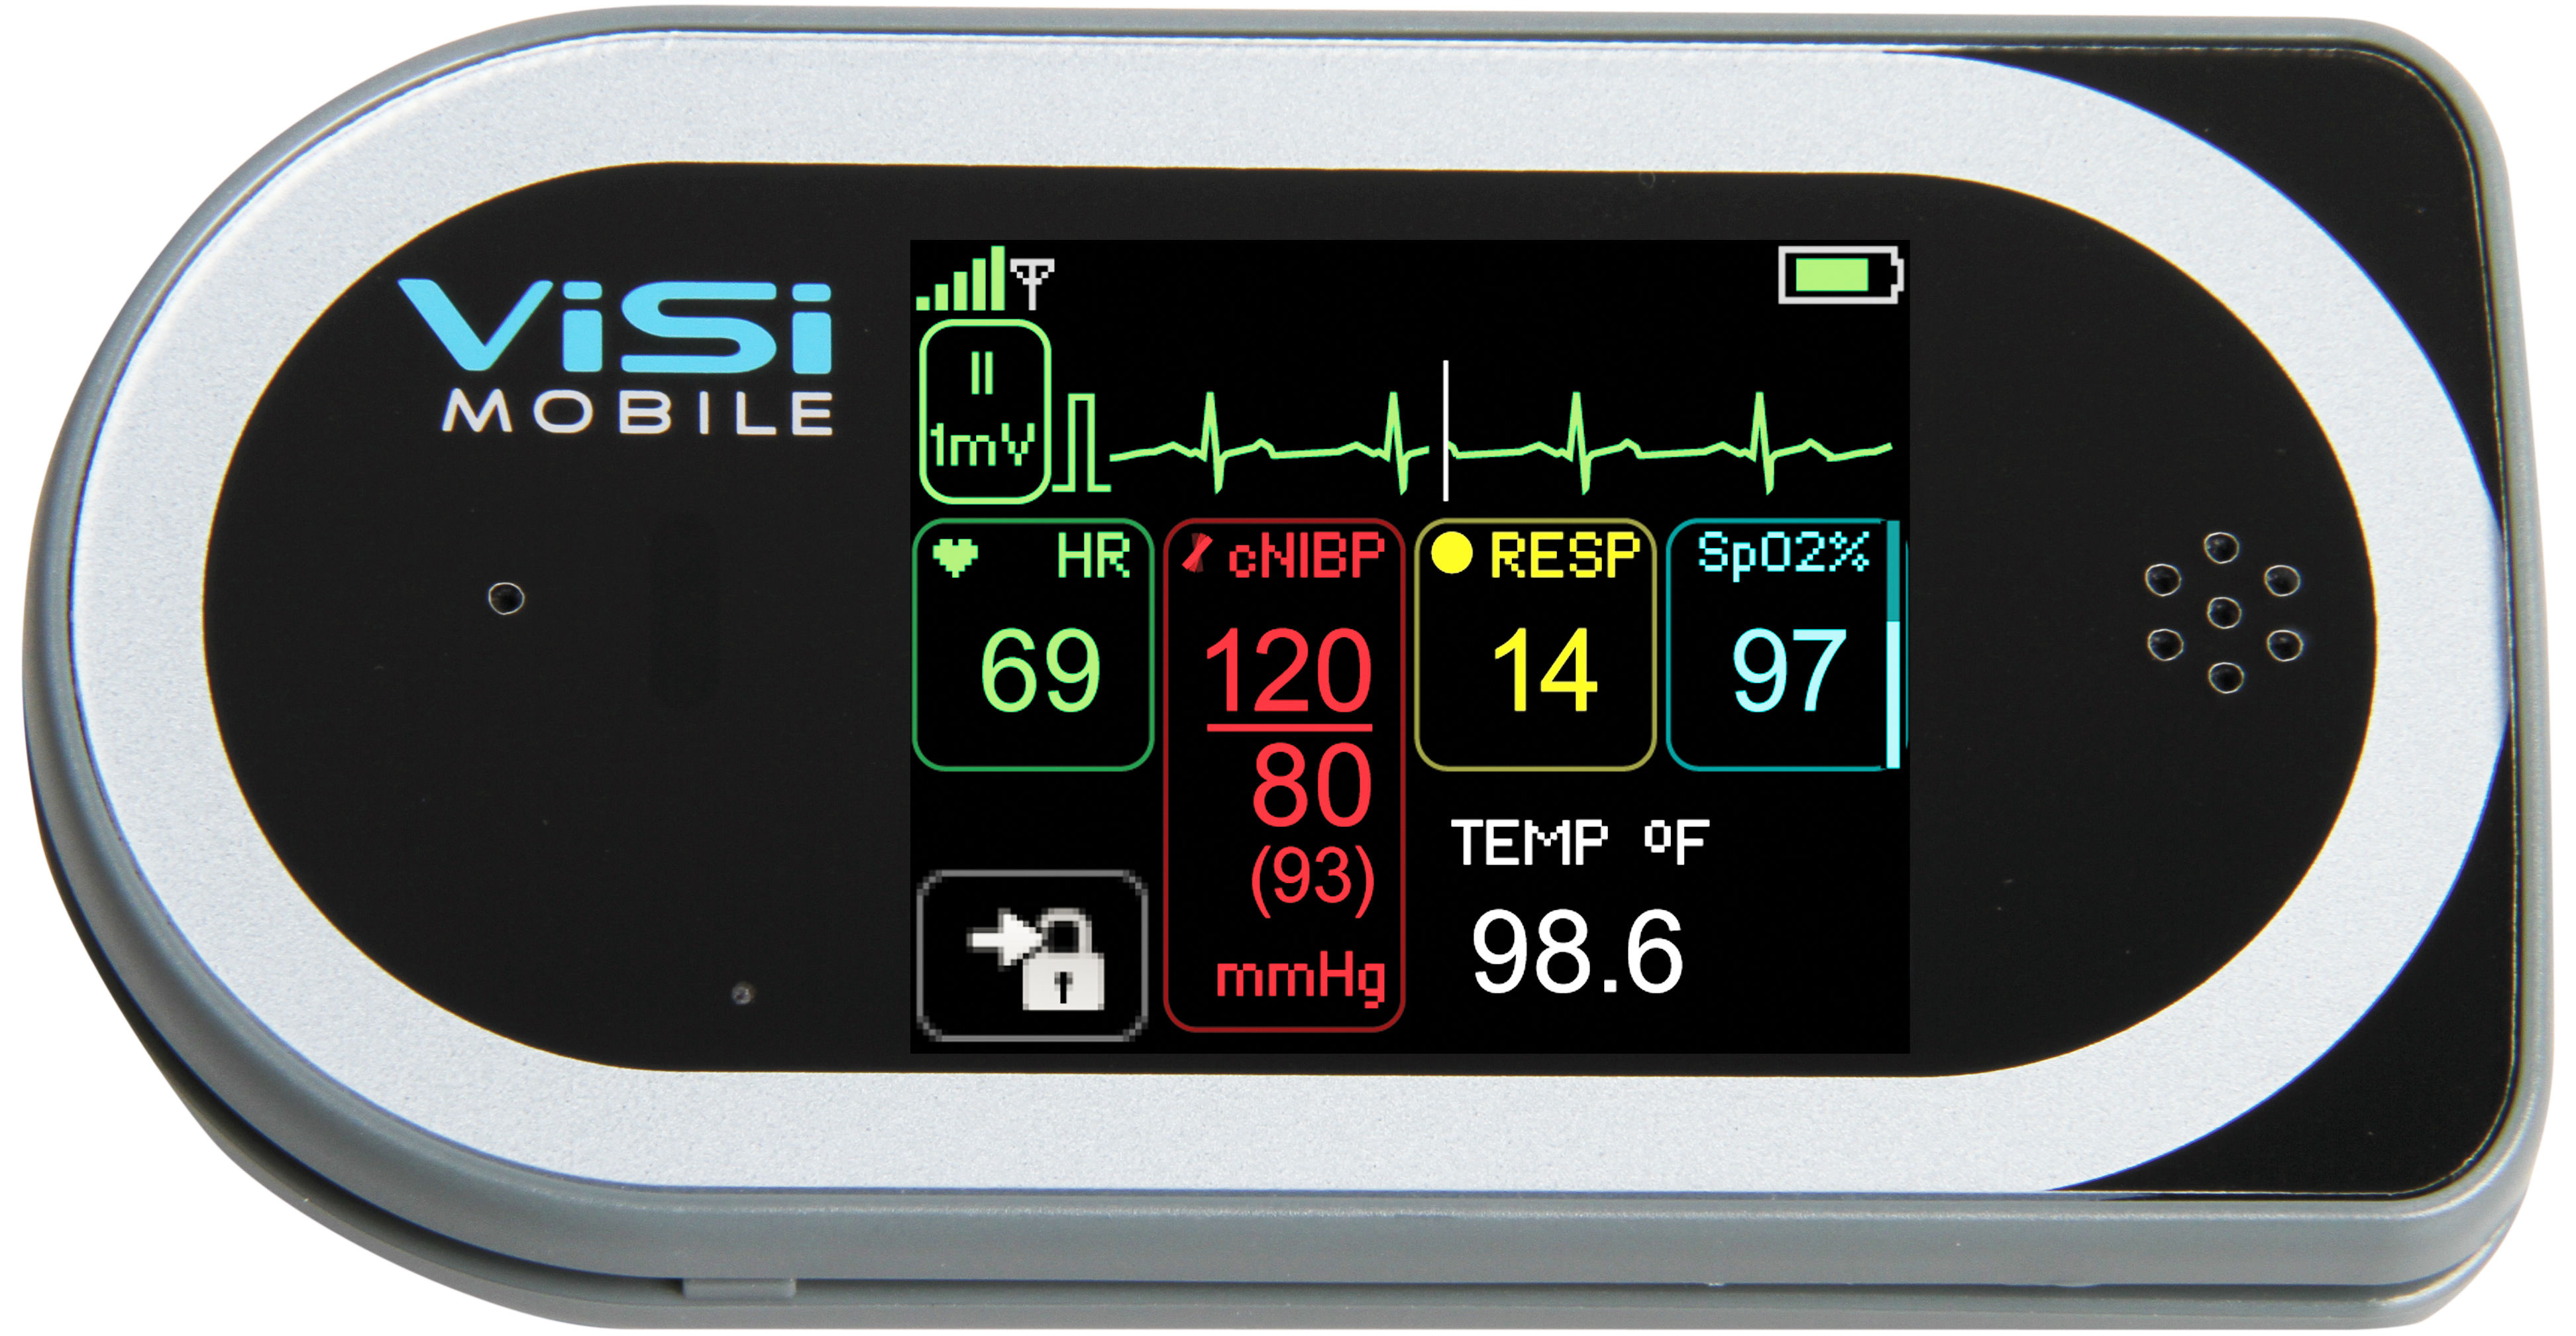
\includegraphics[scale=0.3]{figuras/estadoarte/visi/visi.jpg}
	\caption{Interfaz de usuario ViSi Mobile\textregistered}
	\label{visi1}
\end{figure}

Se puede observar en la figura \ref{visi1} la interfaz que puede ver el paciente al utilizar el dispositivo.

\begin{figure}[H]
	\centering
	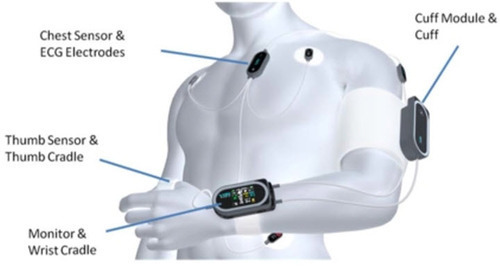
\includegraphics[scale=0.7]{figuras/estadoarte/visi/wear.jpg}
	\caption{Modo de uso ViSi Mobile\textregistered}
	\label{visi2}
\end{figure}

En la imagen de la figura \ref{visi2} se puede observar los sensores conectados al cuerpo que convergen al dispositivo que toma las señales.

\section{Qardiocore\textregistered}

QardioCore\cite{qardio} es un monitor de electrocardiograma inalámbrico diseñado para mejorar la detección y manejo de las condiciones cardíacas. Seis sensores se encargan de grabar y analizar sobre 20 millones de puntos de datos durante todo el día junto con otros signos vitales. Este dispositivo está orientado a personas con alto nivel de riesgo cardíaco causado por predisposición familiar, historial de ataques al corazón, presión alta, colesterol alto, diabetes o exceso de peso. Monitorea de forma precisa y continua la salud del corazón. El dispositivo graba datos de ECG, pulso, variación de pulso, temperatura corporal, ritmo respiratorio y niveles de estrés. A diferencia de los ECG tradicionales, QardioCore no utiliza gel ni cables para monitorear y funciona entre -20ºC y 60ºC. Adicionalmente es resistente al agua y su batería dura alrededor de un día. Respecto a las especificaciones técnicas, es capaz de funcionar con una frecuencia de 600 muestras por segundo y una resolución de 16 bit, apoyándose en comunicación Bluetooth 4.0 y plataforma exclusiva iOS (9.0 o superior)\cite{qardio_tel}.

\begin{figure}[H]
	\centering
	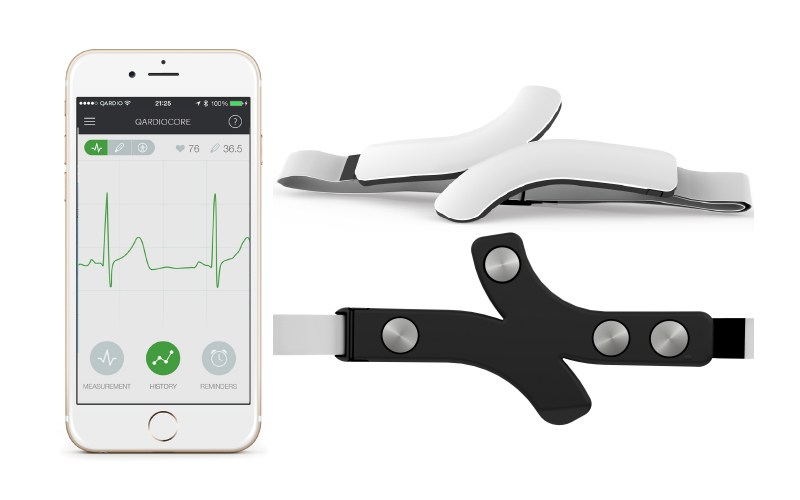
\includegraphics[scale=0.5]{figuras/estadoarte/qardio/qardio.jpg}
	\caption{Qardiocore multisensor}
	\label{qardio1}
\end{figure}

Se puede observar el dispositivo Qardiocore en la figura \ref{qardio1} que se conecta a un smartphone para mostrar los datos que se están tomando.

\newpage
Además como se muestra en la figura \ref{qardio2} es de simple uso, funciona como un cinturón en el pecho del paciente.

\begin{figure}[H]
	\centering
	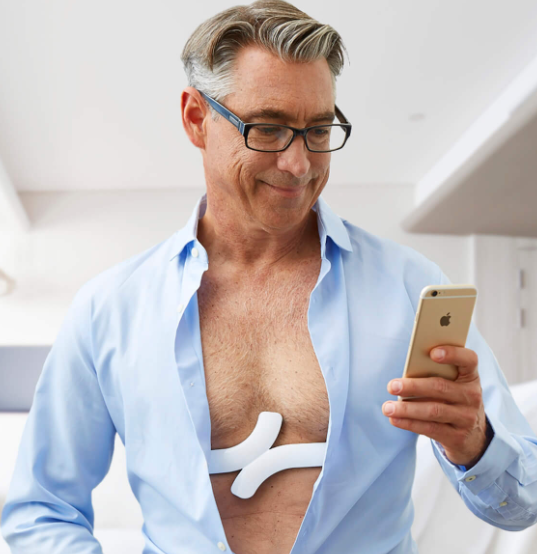
\includegraphics[scale=0.5]{figuras/estadoarte/qardio/wear.png}
	\caption{Modo de uso Qardiocore}
	\label{qardio2}
\end{figure}

\section{Nuubo\textregistered}

Nuubo\cite{nuubo} proporciona una nueva perspectiva en la monitorización cardiológica remota e inalámbrica. La plataforma de Nuubo, nECG platform, permite la captura del ECG dinámico a través de un innovador sistema que está basado en textiles biomédicos de nueva generación, y es rentable, remoto, continuo y no invasivo. Además, puede ser utilizado simultáneamente con uno o varios pacientes. Se basa en tecnología Bluetooth v2.0 + EDR (PC y móvil), con una frecuencia de 250 muestras por segundo y 12 bit de resolución\cite{nuubo_tel}.
La tecnología de electrodos textiles desarrollada por Nuubo simplifica enormemente los incómodos procedimientos tradicionales de conexión de electrodos, reduciéndolos al sencillo acto de vestir la camiseta nECG SHIRT que se muestra en la figura \ref{shirt}.

\begin{figure}[H]
	\centering
	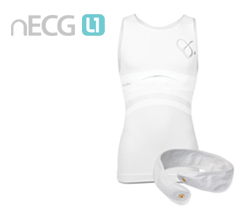
\includegraphics[scale=0.6]{figuras/estadoarte/nuubo/shirt.png}
	\caption{nECG Shirt}
	\label{shirt}
\end{figure}

El tejido elástico se adapta a los movimientos del paciente, quien puede realizar su actividad física diaria sin estar limitado por cables y sin necesidad de depender de personal médico especializado. Estas características junto con la información de contexto, la actividad física del paciente y su posición/postura, permite el desarrollo de un nuevo rango de soluciones y casos de uso. 

\begin{figure}[H]
	\centering
	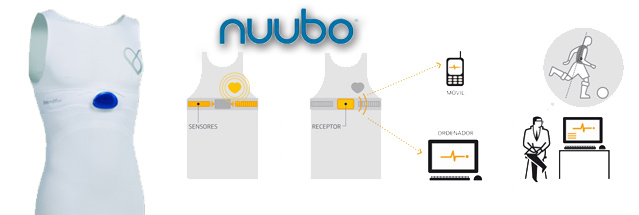
\includegraphics[scale=0.7]{figuras/estadoarte/nuubo/nuubo.png}
	\caption{Sistema Nuubo}
	\label{nuubo}
\end{figure}

Como se puede observar en la figura \ref{nuubo} la polera toma los datos que son enviados a un dispositivo movil o un computador para que sea visto por el doctor de manera remota.

%Capítulo 3: Arquitectura de la solución
\newpage
\chapter{Arquitectura de la solución}\label{arquitectura}
El ECG (Electrocardiograma) detecta señales del cuerpo gracias a electrodos que se colocan en la superficie del cuerpo, usualmente acompañados de un gel conductor que elimina interferencia de los músculos, fuente de alimentación,  ruido externo, etc. Para que se obtenga una señal de ECG sin distorsiones excesivas, es necesario diseñar filtros que eliminen interferencias antes de analizar la información. \\

\section{DFRobot Heart Rate Monitor}\label{reqfuncional1asc}
El monitor de actividad cardíaca de la empresa DFRobot consiste en una placa que consta de un chip AD8232 en su PCB, el cual provee una clara señal de los intervalos PR y QT (Ver Figura \ref{onda})  de un electrocardiograma. Este entrega un valor análogo que puede ser leído por Arduino y con un conversor análogo-digital interpretarse en forma de gráfico.\\

\begin{figure}[H]
\centering
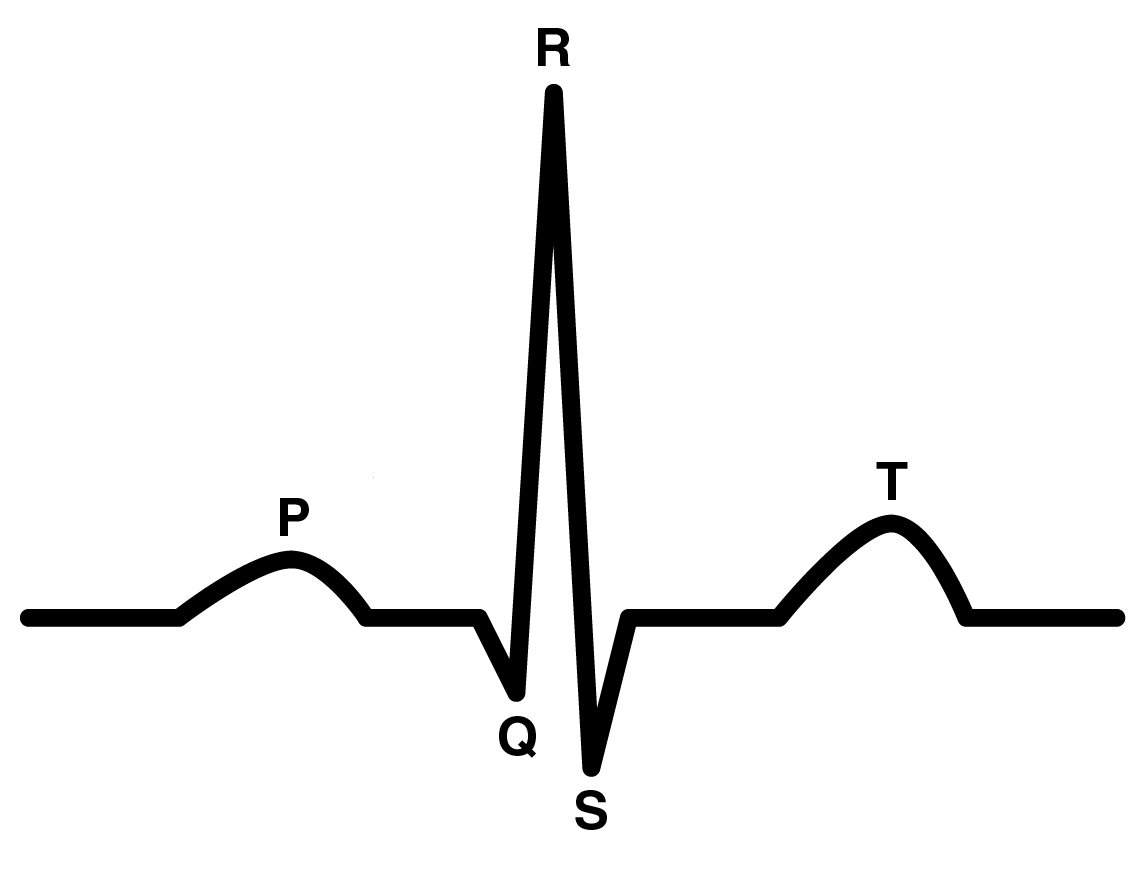
\includegraphics[scale=0.2]{figuras/ecg/senal.png}
\caption{Forma de onda teórica ECG}
\label{onda}
\end{figure}

Se escogió esta placa de desarrollo por disponibilidad de hardware, ya que es la única opción disponible de bajo costo, y que no necesita comprarse fuera del país. Por lo que se tomó la decisión de estudiar su funcionamiento, replicarlo para el diseño del dispositivo final y evaluar posibles mejoras. \\

\section{Biopac MP150 ECG100C}
Se tuvo la oportunidad de usar el ECG de la empresa Biopac ECG100C, el cual es de mucho mayor costo y tamaño utilizado generalmente para investigación. La idea era ver la forma de onda y comparar las frecuencias de corte utilizadas. La figura \ref{biopac} muestra el aparato encargado de tomar las señales de los electrodos y la figura \ref{frecuencias} muestra un acercamiento con las posibles frecuencias de corte configurables para los filtros.\\

\begin{figure}[H]
\centering
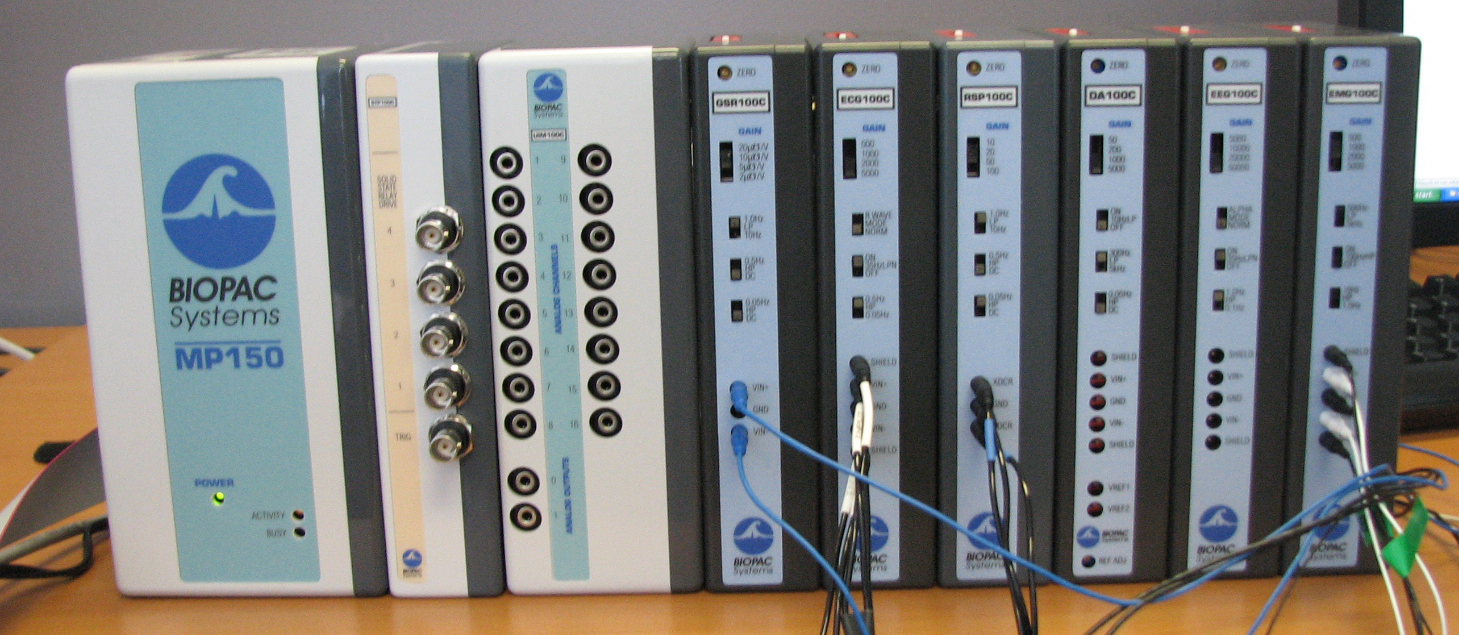
\includegraphics[scale=0.7]{figuras/ecg/biopac.jpg}
\caption{Biopac MP150}
\label{biopac}
\end{figure}

\begin{figure}[H]
\centering
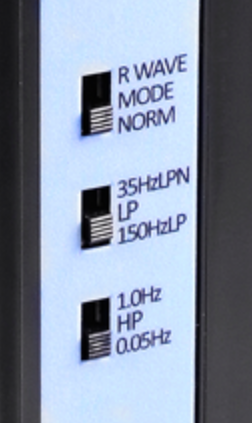
\includegraphics[scale=0.7]{figuras/ecg/biopacecg.png}
\caption{Frecuencias de corte disponibles en Biopac ECG100C}
\label{frecuencias}
\end{figure}

Cabe destacar el alto precio de este equipo que es de 45.000 USD y grandes dimensiones ya que está diseñado para investigación lo cual servirá para saber donde tiene que apuntar la forma de onda de un ECG de grado médico.\\

\newpage
\section{AD8232}
El chip AD8232 es un integrado que permite medir las señales de los electrodos del ECG mediante amplificadores operacionales como se muestra en la figura \ref{ad8232}.

\begin{figure}[H]
\centering
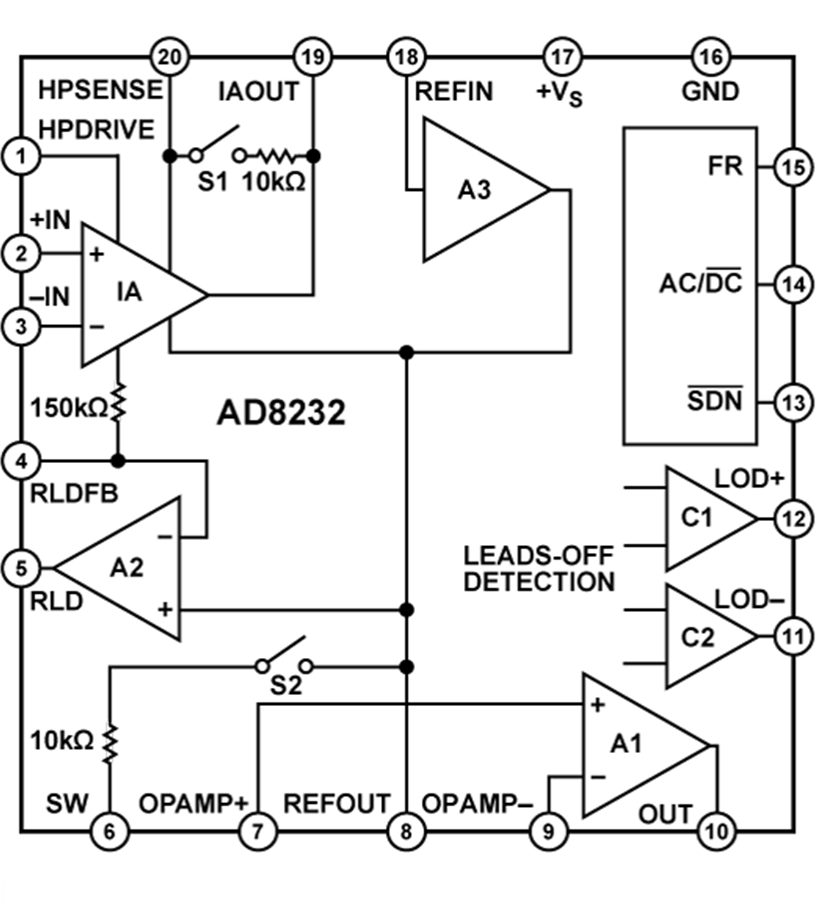
\includegraphics[scale=0.4]{figuras/ecg/ad8232.png}
\caption{Diagrama de bloques funcional}
\label{ad8232}
\end{figure}

Esta figura representa el funcionamiento del integrado y el proceso que realiza en su interior desde el punto de vista de los pines. 
A partir de este diagrama y la herramienta que provee el fabricante para el diseño de filtros, se puede llegar a una configuración del integrado con componentes pasivas para el diseño del circuito impreso como se muestra en la figura \ref{ecgdesign}.\\

\begin{figure}[H]
\centering
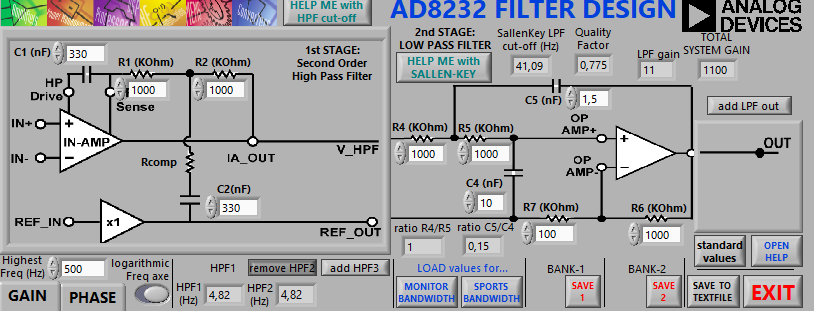
\includegraphics[scale=0.6]{figuras/ecg/ecgdesign.png}
\caption{Herramienta para diseño de filtros}
\label{ecgdesign}
\end{figure}

Como se puede observar en la figura \ref{ecgdesign}, en el lado izquierdo se diseña un filtro pasa alto de segundo orden cuya frecuencia de corte es de 4.82[Hz]. A la derecha se muestra un filtro pasabajo sallen-key con frecuencia de corte 41.09[Hz] donde finalmente se tiene una salida hacia el Arduino. 
Estos valores se obtuvieron al ver el circuito de la PCB de DFRobot (Figura \ref{esquematico11}) y utilizando la herramienta de diseño de filtros. En caso de que se quisieran cambiar las frecuencias de corte se podría hacer un nuevo diseño utilizando el mismo programa pero cambiando y apuntando a frecuencias de corte entre 1-35[Hz] dadas por el dispositivo Biopac.

\begin{figure}[H]
\centering
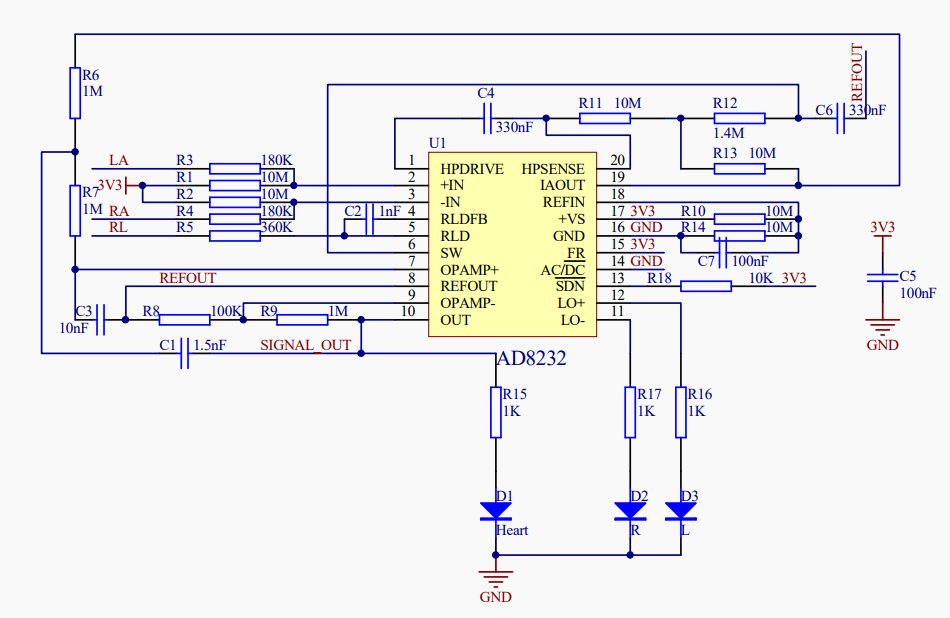
\includegraphics[scale=0.45]{figuras/ecg/esquematico.png}
\caption{Esquemático ECG DFRobot}
\label{esquematico11}
\end{figure}

\newpage
\section{Comparación entre Biopac y DFRobot}
Finalmente se pudo contrastar ambas señales, se puede observar en la figura \ref{graficos} la señal de ECG del Biopac y DFRobot colocando los electrodos muy cerca para obtener las señales lo más parecidas posibles y poder compararlas. 

\begin{figure}[H]
\centering
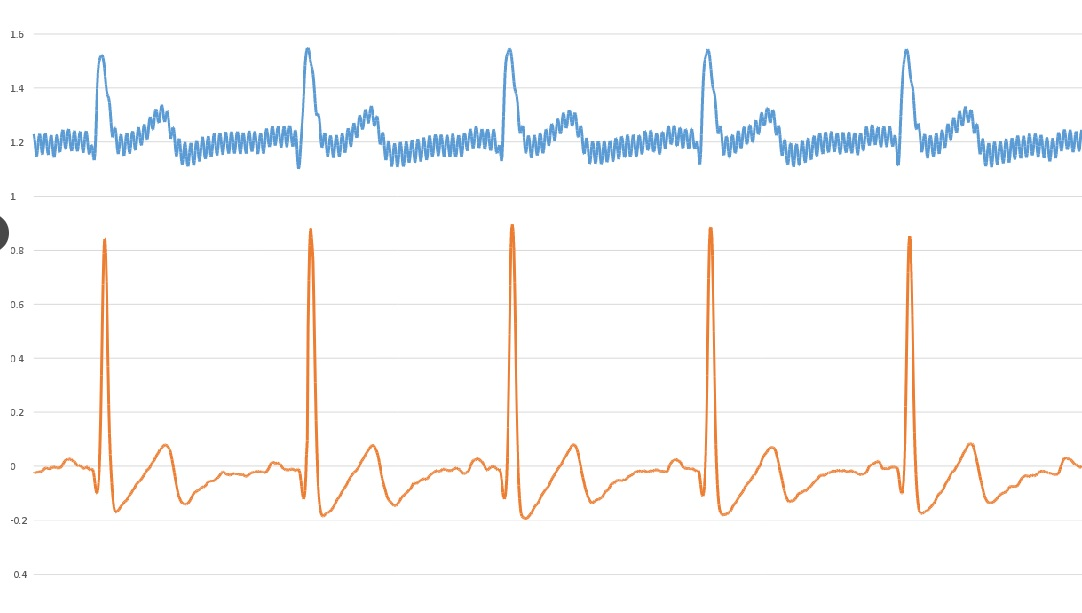
\includegraphics[scale=0.45]{figuras/ecg/biovsdf.jpg}
\caption{Gráfico Biopac ECG100C vs ECG DFRobot}
\label{graficos}
\end{figure}

En el gráfico superior se puede observar la forma de onda del ECG AD8232 en la cual se puede observar notoriamente un ruido de la fuente. En el gráfico inferior se muestra la señal del ECG100C de Biopac, la cual es una señal muy definida a lo cual debería apuntar el diseño del ECG.
Se puede concluir de estas imágenes que la forma de onda de ambas señales son parecidas, considerando que el Biopac está diseñado para mostrar la onda completa, en cambio el AD8232 se encarga de mostrar la onda PR y QT. 
Finalmente se considera que la forma de onda que se tiene sirve para hacer mediciones eliminando el ruido de la fuente ya que es representativa por los peaks que presenta. 

\section{Eliminando ruido de la fuente}
Observando la señal que se tiene actualmente en el dispositivo mediante bluetooth en la aplicación móvil se obtiene una señal como se observa en la figura \ref{ecgfeo}.

\begin{figure}[H]
\centering
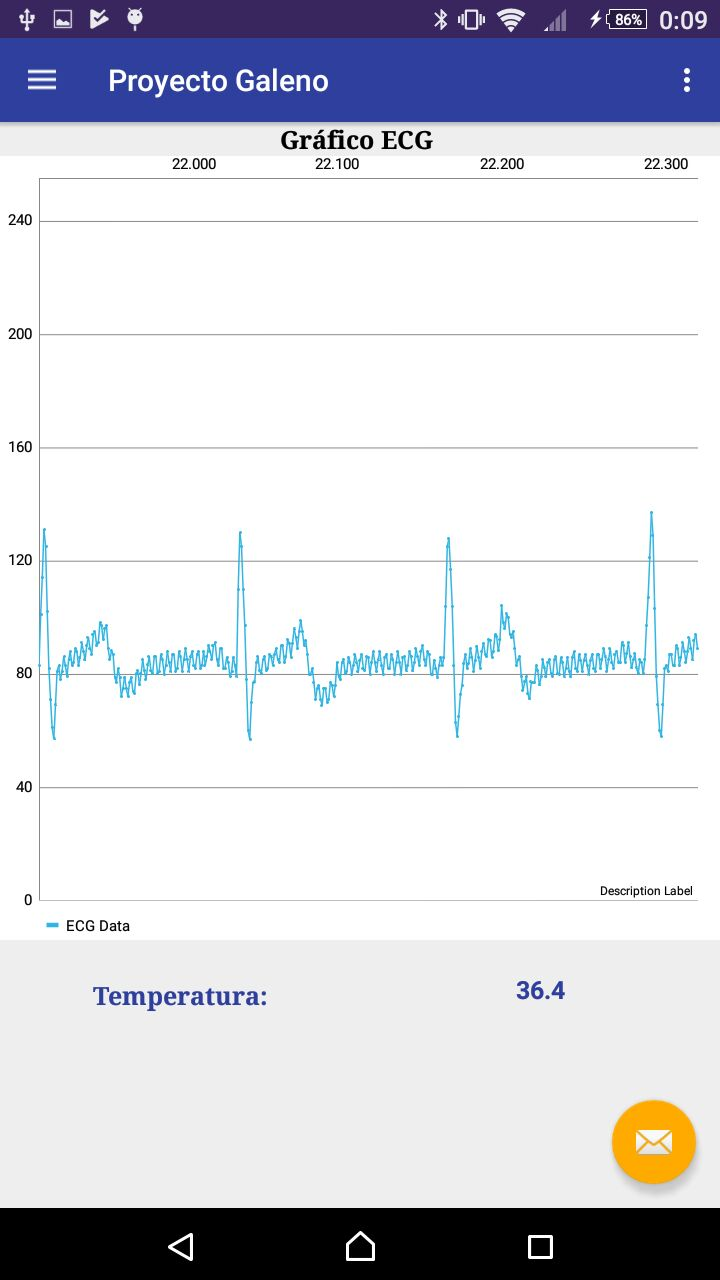
\includegraphics[scale=0.3]{figuras/ecg/ecgappmalo.jpg}
\caption{ECG en aplicación móvil sin filtro de salida}
\label{ecgfeo}
\end{figure}

Se puede notar en esta imagen que la forma de onda se mantiene al enviarla por bluetooth a la aplicación pero sigue con mucho ruido. Utilizando la herramienta de diseño de filtros para el AD8232 existe una opción para filtrar la salida de la señal final, para esto se considera utilizar un filtro pasabajo para eliminar el ruido como se muestra en la figura \ref{filtroout}.

\begin{figure}[H]
\centering
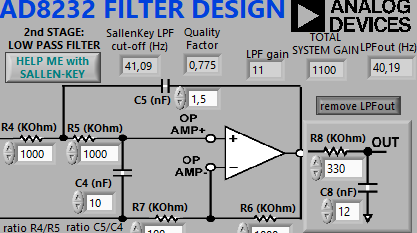
\includegraphics[scale=0.75]{figuras/ecg/filtroout.png}
\caption{Filtgro de salida R8 y C8}
\label{filtroout}
\end{figure}

Se diseñó con frecuencia de corte de $40.19[Hz]$ como se muestra en la figura \ref{filtroout} dando valores $R8 = 330[k\Omega]$ y $C8 = 12[nF]$ para no perder información de la señal y con esto limpiar solamente la señal como se muestra en el resultado de la figura \ref{ecgbonito}

\begin{figure}[H]
\centering
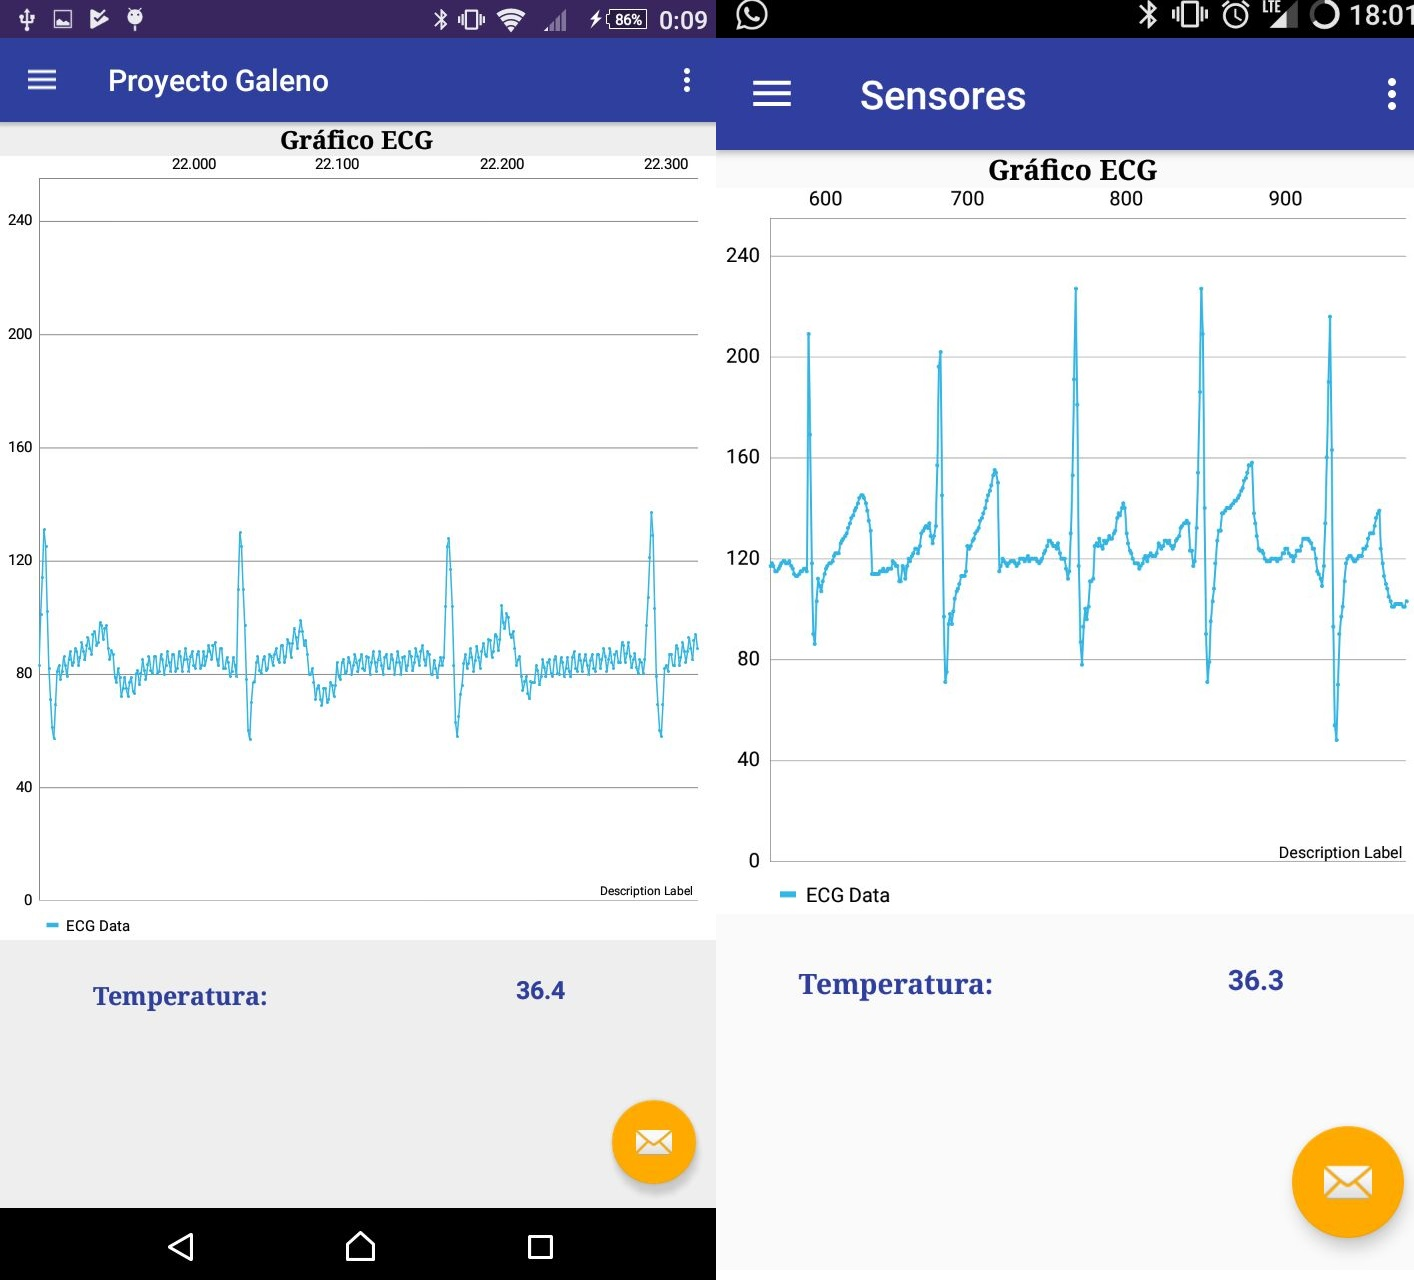
\includegraphics[scale=0.25]{figuras/ecg/ecgappbueno.jpg}
\caption{Comparación ECG en aplicación móvil con filtros de salida}
\label{ecgbonito}
\end{figure}

Se nota un gran cambio en la forma de la señal, donde se notan de mejor manera, sin ruido de la fuente y sin perder la forma de onda. Esta será la configuración que se utilizará para el diseño final del dispositivo.



%Capítulo 4: Alternativas de desarrollo
\newpage
\chapter{Alternativas de desarrollo}\label{alternativas}
La carga de una batería de Li-ion sigue un perfil diseñado para asegurar la seguridad y la vida de estas sin comprometer su rendimiento. Si una batería de Li-ion es descargada completamente, se aplica una precondición de carga de alrededor del 10\%. Esto previene que la pila suba mucho su temperatura hasta un tiempo que sea aceptable enviar 100\% de la corriente hacia la pila como se puede observar en la figura \ref{grafico}.\\
\begin{figure}[H]
\centering
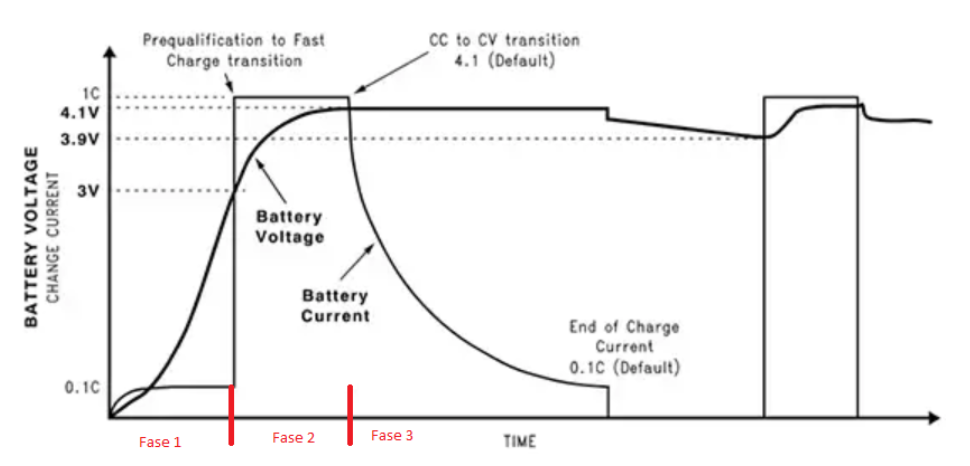
\includegraphics[scale=0.6]{figuras/bateria/grafico.png}
\caption{Etapas de carga de baterías Li-ion para una batería de 4.2[V]}
\label{grafico}
\end{figure}

Como se puede observar en la figura \ref{grafico}, la fase 1 sería la pre-condición de carga del 10\% por un tiempo determinado, luego entra a la fase 2 de corriente al máximo constante y finalmente pasa a la fase 3 donde se mantiene un voltaje constante mientras cae la corriente hasta que termina la carga. 
Cabe destacar que las corrientes se miden en términos de la variable ``C`` la cual se refiere a la corriente que provee la batería, por ejemplo, una batería de $950[mA]$ posee un $C=950$. Esto es importante definir para poder realizar los cálculos de las distintas etapas en el proceso de carga.
\section{Cargador de batería con corriente compartida con carga}
En la actualidad, todos los dispositivos electrónicos tienden a ser lo mas simple posible, es por esto que los diseños que se usan ahora poseen una batería interna que no se puede cambiar o no se deban sacar para cargarlas y así facilitar la tarea al usuario. \\
Esto puede causar un problema debido a la pre-condición que existe en la fase 1 de la figura \ref{grafico}. Si el sistema empieza a pedir mucha corriente implicaría que pueda que no se cumpla esa condición y en ese caso la carga (Arduino) estaría descargando la batería en vez de permitir que se cargue, es por esto que existen integrados que pueden otorgar funcionamiento que permite la interacción de estos.\\
\section{MCP73871}
Considerando un integrado de microchip, el MCP73871\cite{bateria} otorga una funcionalidad de diseñar un sistema que se encargue de cargar una batería de Li-ion con un sistema conectado, que en este caso sería el Arduino. En la tabla \ref{pinesmcp} se muestra la descripción de los pines que se utilizarán en el diseño.\\

\begin{table}[H]
\centering
\begin{tabular}{| c | c | c |}
\hline
\multicolumn{1}{|c|}{\textbf{Nº Pin}}&
\multicolumn{1}{c|}{\textbf{Nombre}}&
\multicolumn{1}{|c|}{\textbf{Función}}\\ \hline
1, 20 & Out & Salida hacia la carga\\ \hline
18, 19 & In & Entrada alimentación\\ \hline
13 & PROG1 & Regulación de corriente de carga rápida\\ \hline
3 & SEL & Selección de input\\ \hline
4 & PROG2 & Límite de corriente entrada USB\\ \hline
12 & PROG3 & Corriente de término de la carga\\ \hline
14, 15 & VBAT & Conexión positiva con la batería\\ \hline
16 & VBAT\_ SENSE & Sensor de voltaje de la batería\\ \hline
\end{tabular}
\caption{Descripción de pines MCP73871}
\label{pinesmcp}
\end{table}

\subsection{Power Supply Input (IN)}
Este viene a ser la conexión a la alimentación en la cual se puede usar un adaptador a la pared USB además de poder cargarlo con un computador. Cuando se usa con la pared se debe considerar que el rango de voltaje debe estar entre $V_{bat} +300[mV]$ y $6[V]$. En este caso no habría problema ya que esta conexión USB provee $5[V]$ y la batería que se va a utilizar es de $3.6 [V]$.

\subsection{Input Source Type Selection (SEL)}
Este pin cumple una función de selección para carga rápida. Con una entrada lógica baja, el limite de carga es de baja corriente $100[mA]$, en cambio al utilizar una entrada lógica alta, la entrada de corriente llega a ser de $500[mA]$. Este pin tiene una relación con la selección del nivel lógico que tenga el pin ''SEL'' como se puede observar en la figura \ref{cargarapida}.\\
\begin{figure}[H]
\centering
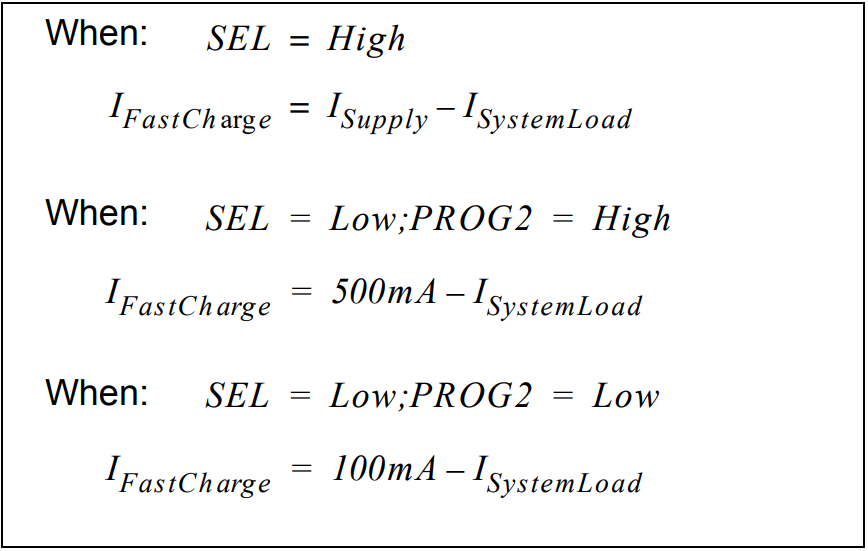
\includegraphics[scale=0.5]{figuras/bateria/cargarapida.png}
\caption{Configuraciones disponibles para carga rápida}
\label{cargarapida}
\end{figure}

Como se puede observar al utilizar ''SEL'' conectado a tierra permite que ''PROG2'' pueda ser utilizado cargando a $500[mA]$ o $100[mA]$ por lo que se elegirá la entrada de ''PROG2'' en alto para que se permita de igual manera cargar rápido y utilizar todas las funciones del dispositivo dejando un límite de seguridad de $500[mA]$.

\subsection{Regulación de carga rápida(PROG1)}
El pin ''PROG1'' determina el máximo constante de corriente con un resistor entre el pin 13 y tierra. Este además fija el máximo de corriente permitida y la corriente de término. Para calcular se debe considerar la ecuación \ref{ivsR}.

\begin{equation}\label{ivsR}
I_{carga} = \frac{1000[V]}{R_{PROG1}[k\Omega]}
\end{equation}

Primero se debe conocer la corriente de carga $I_{Carga}$, para esto se utiliza la ecuación  \ref{calculoRPROG}.
\begin{equation}\label{calculoRPROG}
R_{PROG1} = \frac{1000[V]}{I_{carga}} = 1.315[k\Omega] \approx 1.3[k\Omega]
\end{equation}

Despejando esta ecuación se obtiene un resultado aproximado de $1.3[k\Omega]$ que será la resistencia utilizada para el diseño

\subsection{Corriente de término de carga (PROG3)}

El ciclo de carga es terminado cuando, durante una etapa de voltaje constante (Figura \ref{grafico}), el promedio de corriente disminuye un límite (generalmente 0.1C) que se fija con un resistor conectado desde el pin ''PROG3'' hasta $V_{ss}$ el cual puede ser conectado a tierra.

\begin{equation}\label{Rprog3}
R_{PROG3} = \frac{1000[V]}{I_{Termino}} = 10.5[k\Omega] \approx 10[k\Omega]
\end{equation}

\subsection{Salida de voltaje a la batería $V_{BAT}$ y sensor de voltaje de batería $V_{SENSE}$}

Al conectar el terminal positivo de la batería de Li-ion el pin  $V_{BAT}$ cumple la función de cargarla, es recomendable utilizar un capacitor de cerámico en la salida para que asegure la estabilidad de la carga. 
El pin $V_{SENSE}$ se encarga de entregar el voltaje de salida para que el integrado se pueda realimentar con el valor que está entregando y corregirlo. 

\subsection{Pines Generales}

Los pines mencionados anteriormente son los más relevantes con respecto a diseño del dispositivo, hay otros pines que recomienda el fabricante utilizar como referencia para el usuario o el desarrollador los cuales muestran, conectando diodos led, Estado de batería, estado de carga y si se está entregando o no alimentación al dispositivo. 
Además hay otras funciones que no se utilizan por lo que esos pines son conectados a tierra o al voltaje de alimentación según se especifique.

\subsection{Diseño del esquemático}

Con todos los cálculos anteriores, finalmente se diseña el circuito con el integrado en el programa EagleCAD que será usado para enviar a producción de la PCB como se muestra en la figura \ref{esquematico22}.

\begin{figure}[H]
\centering
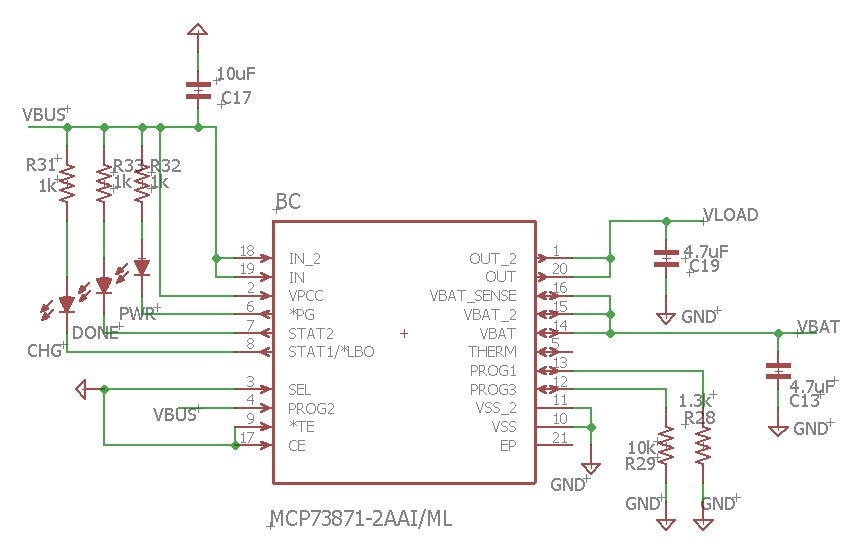
\includegraphics[scale=0.7]{figuras/bateria/esquematico.jpg}
\caption{Diseño de cargador de batería en software EagleCAD}
\label{esquematico22}
\end{figure}

Se puede observar los valores diseñados para una batería de $3.7[V]$ de Li-ion con $950[mAh]$ de capacidad. Como se recomendó en $V_{BAT}$ es necesario utilizar condensadores de cerámica para regular las salidas, al igual que en $V_{LOAD}$ el cual viene a ser el que se entrega al Arduino.\\
Se eligen los valores de ''SEL'' en $0[V]$ y ''PROG2'' en $5[V]$ para así limitar la corriente de carga a la diferencia entre $500[mA]$ y la corriente de la carga, tal como se indica en la figura \ref{cargarapida}.

%Capítulo 5: Sistema de telecomunicaciones
\newpage
\chapter{Sistema de telecomunicaciones}\label{comunicacion}
Se determinó utilizar la plataforma Arduino por su simplicidad en prototipado y programación, además de ser de fácil acceso y una tecnología escalable.
\section{ATMega328p}
Utilizando una placa Arduino Uno se comienza el prototipo del dispositivo que va a cumplir la función de tomar los datos de los sensores análogos. La versión de Arduino Uno utiliza un microcontrolador ATMega328 que posee 32[KB] de memoria de programa y una memoria RAM de 2[Mb]. Este consta de 1 puerto de comunicación UART y posee 32 pines de los cuales 23 pines son programables para entrada/salida como se muestra en la figura \ref{328}

\begin{figure}[H]
\centering
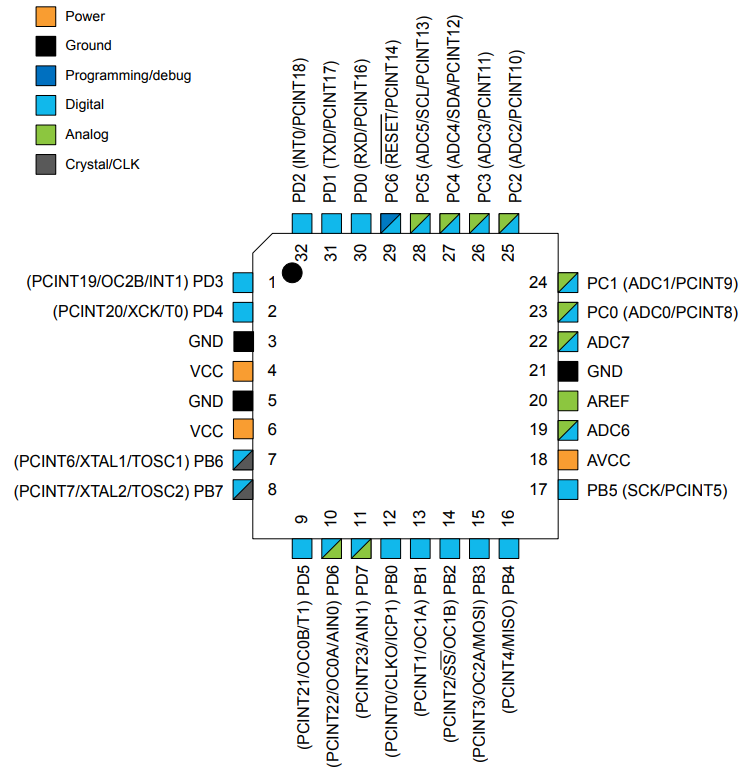
\includegraphics[scale=0.35]{figuras/mcu/328.png}
\caption{Microcontrolador ATMega328p}
\label{328}
\end{figure}

\section{ATMega2560}
Contrastando el modelo mostrado anteriormente, la placa Arduino Mega posee un microcontrolador ATMega2560 el cual incluye un aumento en todas sus capacidades. Comenzando con la capacidad de su memoria de programa, que asciende a 250[KB] y una memoria RAM de 8[KB]. Este microcontrolador posee 100 pines lo que incluye un aumento a 4 puertos de comunicación UART, además de aumento de entradas análogas y digitales. 

\begin{figure}[H]
\centering
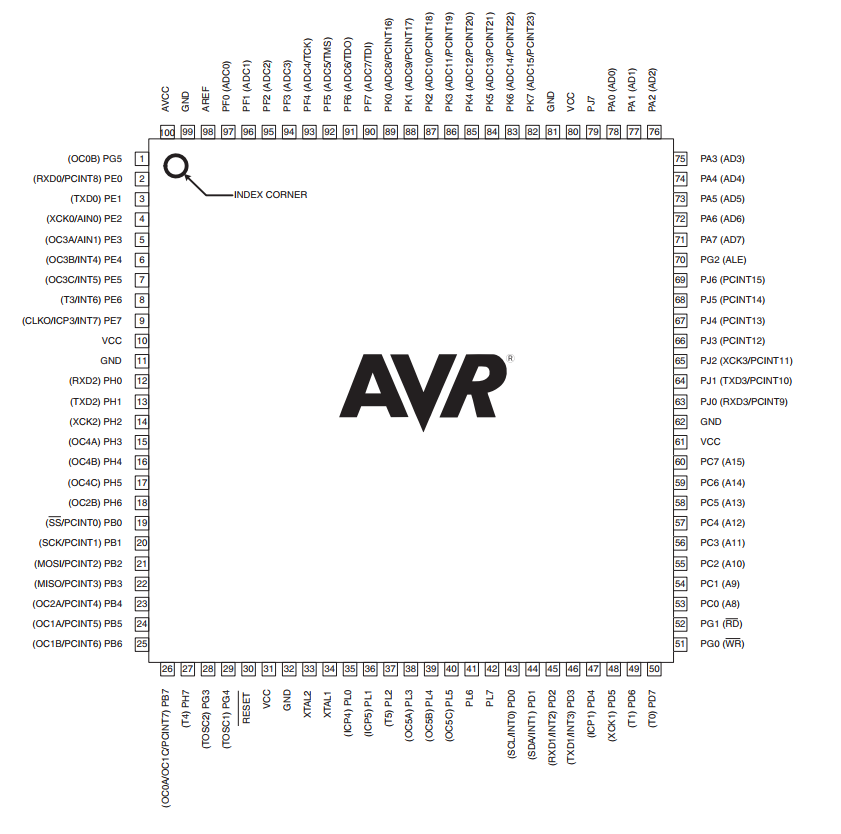
\includegraphics[scale=0.5]{figuras/mcu/2560.png}
\caption{Microcontrolador ATMega2560}
\label{mega}
\end{figure}

Como se puede observar en la figura \ref{mega}, hay un aumento considerable en las prestaciones que ofrece este microcontrolador con respecto al ATMega328p además de su tamaño. \\

Se va a trabajar en el diseño con este microcontrolador ya que posee 4 interfaces UART de las cuales una de estas siempre está definida para ser utilizada por la programación FTDl, esto se explicará mas adelante.\\

Esto involucra utilizar un chip con mayores capacidades de las necesarias pero esto es debido a la limitante de los microcontroladores utilizados por Arduino como se puede observar en la figura \ref{compara}.

\begin{figure}[H]
\centering
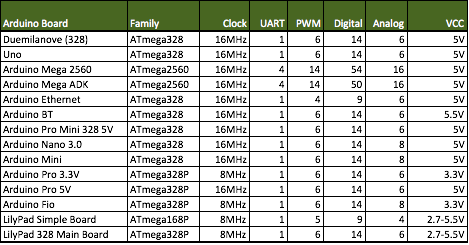
\includegraphics[scale=0.7]{figuras/mcu/compara.png}
\caption{Comparación microcontroladores Arduino}
\label{compara}
\end{figure}

Idealmente para el diseño del dispositivo, se utilizará un microcontrolador con 2 puertos UART ya que uno de estos es necesario para la comunicación con el computador y el otro es utilizado para el envío de información mediante bluetooth, pero por necesidad de rapidez para el diseño de prototipo y pruebas de sensores es necesario iterar con una placa ya fabricada para usos generales y disponibles en el mercado. Esto causaría una disminución significativa entre el precio del diseño del producto final. 
\newpage
\section{ATMega644PA}
Considerando la variable de costos es importante destacar una tercera opción para el diseño del dispositivo final. El microcontrolador ATMega644PA posee un menor conteo de pines ya que consta de 44 lo cual disminuye costos y tamaño a la hora del diseño. Con una memoria Flash de 64[KB] y memoria RAM de 4[KB]. Este provee 2 UART para la comunicación y los pines suficientes para sensores como se muestra en la figura \ref{644}.

\begin{figure}[H]
\centering
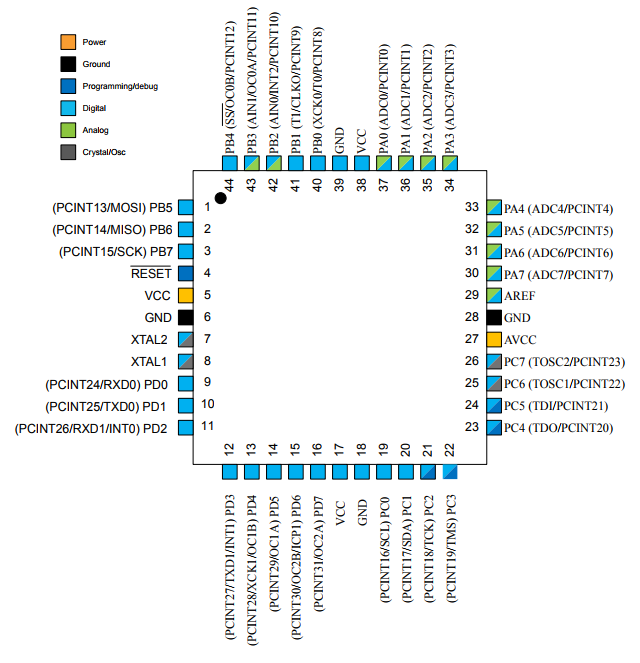
\includegraphics[scale=0.7]{figuras/mcu/644.png}
\caption{Microcontrolador ATMega644PA}
\label{644}
\end{figure}

Se puede observar en la imagen la disponibilidad de los puertos UART donde el Pin 9 y Pin 10 corresponden a UART0 considerado para la programación USB. Pin 11 y Pin 12 corresponden a UART1 que será utilizado para la comunicación con el dispositivo bluetooth.\\
En primera instancia se va a diseñar el dispositivo con el microcontrolador ATMega2560, debido a que existen modelos Arduino con esta misma componente y cumple los requisitos funcionales de poseer mas de 1 puerto UART. No es la opción ideal ya que posee mas prestaciones de las que se necesitan pero permite que se pueda prototipar inmediatamente  utilizando un Arduino equivalente, lo cual no se puede hacer con la versión ATMega644PA.

\section{Conclusiones}
Finalmente considerando las 3 opciones elegidas, se puede establecer una decisión final con respecto a cual microcontrolador utilizar.


\begin{table}[H]
\centering
\begin{tabular}{| c | c | c |}
\hline
\multicolumn{1}{|c|}{\textbf{Microcontrolador}}&
\multicolumn{1}{c|}{\textbf{Pines}}&
\multicolumn{1}{|c|}{\textbf{Precio (USD)}}\\ \hline
ATMega328p  & 32  & \$2.18  \\ \hline
ATMega2560  & 100 & \$12.44 \\ \hline
ATMega644PA & 44  & \$5.24  \\ \hline
\end{tabular}
\caption{Comparación microcontroladores}
\label{tablacompara}
\end{table}

Como se puede observar en la Tabla 1 se tomaron en cuenta los aspectos de tamaño y costos. ATMega328p se considera porque a pesar de que posee un solo puerto UART es posible utilizar otros pines para configurar comunicación serial por software (en comparación con la comunicación por hardware es mucho más lenta) lo cual será muy útil a la hora de hacer pruebas en toma de datos y envío de la información. En cuanto a precio y tamaño es una alternativa ideal ya que minimiza ambos aspectos. \\
La segunda opción siendo la que ofrece más opciones para sensores y memoria programable es excesivo para lo que se necesita desarrollar, pero se acerca más a los requerimientos necesarios que carece el microcontrolador ATMega328p. Esta opción tiene un el precio más elevado de las 3 opciones y por una diferencia considerable, es por esto que se utilizará para la primera versión del diseño final enfocado a tener un mínimo producto viable que funcione de la misma manera que el prototipo.\\
Finalmente la tercera opción siendo la más viable ya que posee un tamaño mucho menor al ATMega2560 y un precio menor a la mitad que este, ofrece todas las capacidades necesarias pero como se muestra en la figura \ref{compara}, no hay en el mercado una placa Arduino con este microcontrolador ni tampoco otra opción que cumpla con el requisito de utilizar 2 UART es por esto que como segunda iteración del producto final se debe buscar un bootloader compatible con el entorno de desarrollo Arduino para el ATMega644PA o trabajar en otra plataforma compatible con ese microcontrolador.




%Capítulo 6: Implementación de la solución de lado del servidor
\newpage
\chapter{Implementación de la solución de lado del servidor}\label{servidor}
Los microcontroladores Arduino son usados en el diseño de sistemas embebidos para distintas funciones. El microcontrolador es un pequeño chip que posee pines con funciones de lectura y escritura, memoria, entradas y salidas. Mientras los microcontroladores han sido usados por décadas, los microcontroladores Arduino son utilizados actualmente ya que permiten ejecutar funciones electrónicas sin necesidad de conocer hardware y software integrado en estos. 
\section{Bootloader}
Dentro de las múltiples definiciones que existen con respecto al bootloader, lo más común es considerarlo como un software o firmware que reside parcialmente en la memoria no volátil del microcontrolador, como la ROM o memoria Flash. \\
En la práctica el bootloader empieza a funcionar justo después de prender el microcontrolador o después de reiniciarlo. \\
Este bootloader va a ser el que va a permitir la programación del circuito con el entorno de desarrollo Arduino (Arduino IDE) manejando de mejor manera la toma de datos por medio de las entradas análogas, el procesamiento y la comunicación.

\newpage
\section{ISP - In-System Programming}
También conocido como programación serial en circuito\cite{isp} (ICSP), es la habilidad de algunos dispositivos lógicos programables, microcontroladores y otros circuitos electrónicos de ser programados mientras están instalados en un sistema completo, no es necesario programar el chip antes de instalarlo en el sistema. Esto permite armar un circuito con todo lo que se desea y programarlo en el circuito impreso.\\
Típicamente los chips que soportan programación ISP tienen circuitería interna que genera el voltaje necesario y permite comunicarse con el programador a través de protocolo serial.
La mayoría de los dispositivos lógicos programables usan una variante del protocolo JTAG para ISP para facilitar la integración con procedimientos automatizados de pruebas.\\
JTAG (Joint Test Action Group) es una interfaz diseñada originalmente para circuitos impresos y es muy útil también como mecanismo para depuración de aplicaciones embebidas, puesto que provee una puerta trasera para acceder al sistema. El módulo de depuración permite al programador corregir errores de código y de lógica de sus sistemas.\\

\begin{figure}[H]
\centering
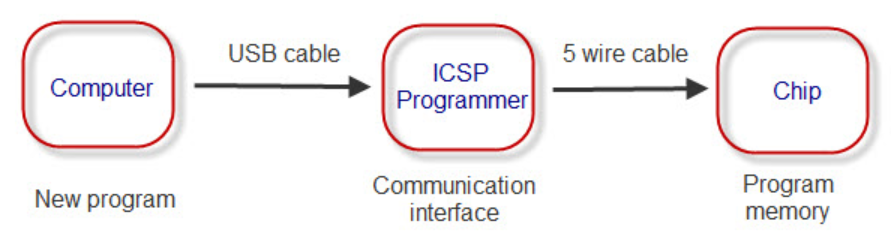
\includegraphics[scale=0.5]{figuras/firmware/isp.png}
\caption{Configuración ISP para programar un microcontrolador}
\label{isp}
\end{figure}

Se observa en la Figura \ref{isp} un simple diagrama de flujo donde es importante destacar que para poder programar un chip es necesaria una conexión de 5 cables entre un intermediario que viene a ser el programador ICSP (o ISP) y el chip (Microcontrolador).

\newpage
\section{Programación de un microcontrolador}
Para que el entorno de desarrollo Arduino reconozca el microcontrolador como una placa Arduino, es necesario grabar el bootloader en este. Se escribe el bootloader en la memoria del microcontrolador mediante la comunicación ISP que se muestra en la figura \ref{pin}.

\begin{figure}[H]
\centering
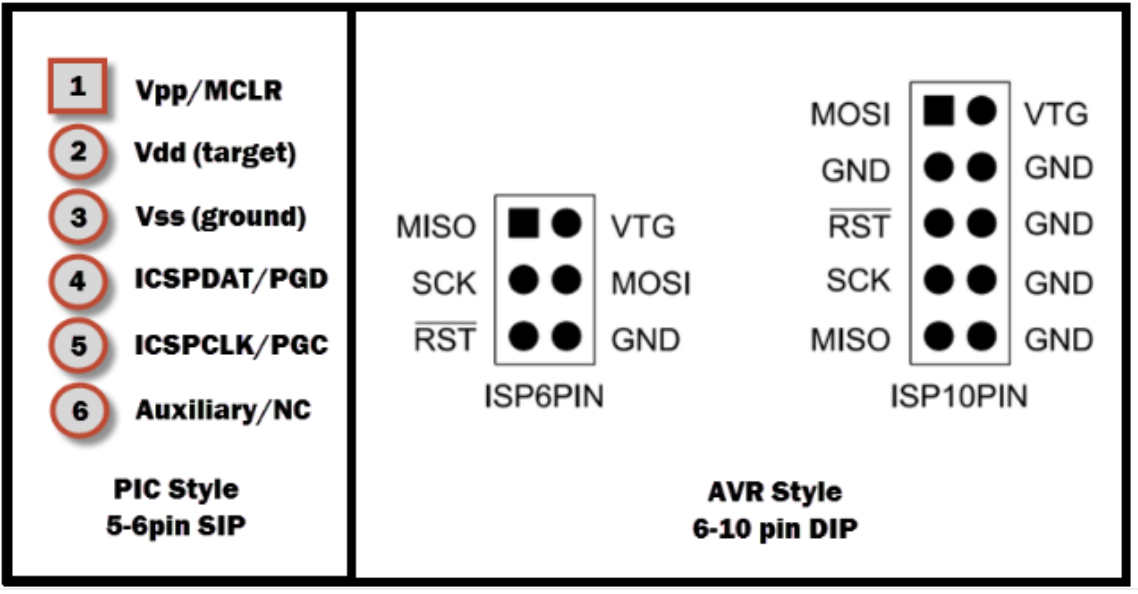
\includegraphics[scale=0.5]{figuras/firmware/pin.png}
\caption{Conector típico para programación ISP}
\label{pin}
\end{figure}

La figura \ref{pin} muestra el conector ISP que se va a encargar de cargar el bootloader en el microcontrolador.  En este caso se está utilizando la tecnología AVR (microcontrolador ATMega) la cual es usada por las placas Arduino y es por esto que se usará la configuración de 6 pines. 

\begin{figure}[H]
\centering
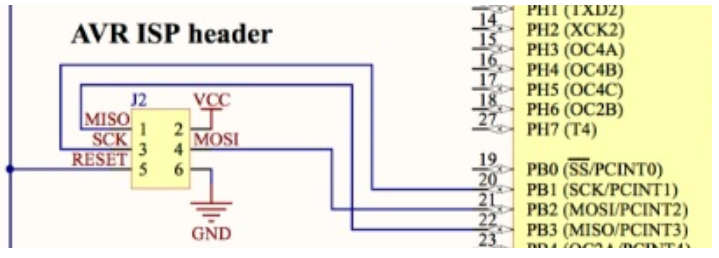
\includegraphics[scale=0.6]{figuras/firmware/eagleisp.png}
\caption{Esquemático básico MCU con ISP}
\label{eagle11}
\end{figure}

En la figura \ref{eagle11} se muestra una parte del esquemático con la configuración básica en el microcontrolador AVR.
Se puede observar el diagrama de conexión del bus con el microcontrolador. Esto se puede observar con mayor detalle en la tabla \ref{tablaisp}\\

\subsection{Programador ISP}
 Existen varias alternativas que cumplen esta función y dependen tanto del microcontrolador como del fabricante. Un microcontrolador AVR (Atmel) requiere de un programador STK500 con una interfaz serial RS232 (Existen otros programadores pero cumplen la misma función, el STK500 es el más utilizado y posee mayor compatibilidad). Para programar un microcontrolador de Microchip se requiere de un PICkit.\\ 
Una segunda alternativa es utilizar un Arduino ya programada que cumpla la función del programador. Estas vienen con un puerto ISP el cual permite cargar el bootloader en el microcontrolador. Respetando la misma conexión que se muestra en la figura \ref{eagle11}.\\

\begin{table}[H]
\centering
\begin{tabular}{| c | c | c |}
\hline
\multicolumn{1}{|c|}{\textbf{AVR ISP}}&
\multicolumn{1}{c|}{\textbf{Arduino UNO}}&
\multicolumn{1}{|c|}{\textbf{ATMega2560}}\\ \hline
1 & MISO  & Pin 22 \\ \hline
2 & VCC   & VCC    \\ \hline
3 & SCK   & PIN 20 \\ \hline
4 & MOSI  & Pin 21 \\ \hline
5 & RESET & Pin 30 \\ \hline
6 & GND   & GND    \\ \hline
\end{tabular}
\caption{Programación ISP utilizando Arduino UNO}
\label{tablaisp}
\end{table}

\section{Programación USB}
La compañía escocesa Future Technology Devices International (FTDI) está especializada en la tecnología USB (Universal Serial Bus). Esta ofrece chips encargados de transformar una conexión USB a un puerto UART y esto será fundamental a la hora de programar el diseño final con el programa en el entorno Arduino.
\newpage
\subsection{FT232RL}
El Chip FT232RL\cite{ft232} ofrece una conversión USB-UART y cuenta con 28 pines como se muestra en la figura \ref{ft232ft}.

\begin{figure}[H]
\centering
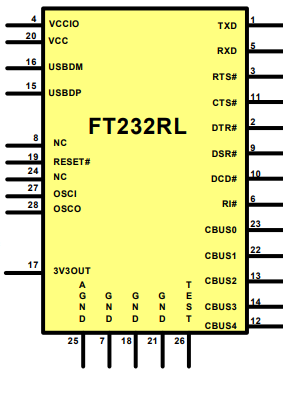
\includegraphics[scale=0.6]{figuras/firmware/ft232.png}
\caption{Chip FT232RL}
\label{ft232ft}
\end{figure}

En la tabla \ref{ft232} se muestra la descripción de los pines más importantes para la conexión del FTDI con el microcontrolador y al mismo tiempo con el USB para permitir la programación del chip. 

\begin{table}[H]
\centering
\begin{tabular}{| c | c | c | c |}
\hline
\multicolumn{1}{|c|}{\textbf{Nº Pin}}&
\multicolumn{1}{c|}{\textbf{Nombre}}&
\multicolumn{1}{|c|}{\textbf{Descripción}}\\ \hline
1  & TXD    & Transmisor de datos UART \\ \hline
5  & RXD    & Receptor de datos UART    \\ \hline
4  & VCCIO  & 1.8[V] a 5.25[V] alimentación a la interfaz UART y a los pines CBUS \\ \hline
15 & USBDP  & Conexión Data+ USB \\ \hline
16 & USBDM  & Conexión Data- USB \\ \hline
17 & 3V3OUT & Regulador de voltaje interno.    \\ \hline
22 & CBUS1  & Indicador de funcionamiento RXD   \\ \hline
23 & CBUS2  & Indicador de funcionamiento TXD    \\ \hline
\end{tabular}
\caption{Descripción de pines chip FT232RL}
\label{ft232}
\end{table}

Este chip será encargado de conectar la interfaz UART (TX y RX) con el microcontrolador además de permitir la comunicación con la conexión USB (USBDP y USBDM).\\
Al trabajar con una conexión USB se tiene conexión con VCC y GND desde el computador que está programando y este provee una alimentación de 5[V]. Este voltaje es comúnmente utilizado en los microcontroladores pero además provee un regulador de voltaje interno de 3.3[V] el cual está disponible si se está trabajando con un sistema con menor voltaje.
En caso de utilizar voltaje 3.3[V] para todo el sistema, es necesario conectar el pin 3V3OUT a VCCIO utilizando un condensador de 100[nF] como se indica en el manual. De esta forma la alimentación del microcontrolador es la misma que la alimentación FTDI para la programación UART y no se dañan las componentes.

\begin{figure}[H]
\centering
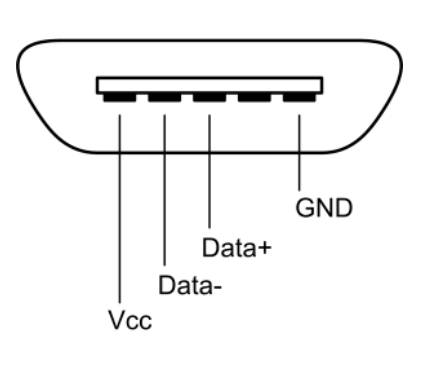
\includegraphics[scale=0.6]{figuras/firmware/usb.png}
\caption{Conector USB 2.0 Micro B}
\label{usb}
\end{figure}

Se muestra en la figura \ref{usb} las 4 conexiones que posee un conector USB, las cuales son la alimentación VCC, GND y la conexión de datos Data+ (USBDP en FT232) y Data- (USBDM en FT232). 

\newpage
\section{Programa en Arduino}

Para la programación del Arduino se trabajó en conjunto con la parte telemática del grupo. Se realizó la programación de la toma de datos de los sensores. Además de un algoritmo antirebote para pedir toma de muestras en el prototipo que luego fue sustituido por una orden emitida por la aplicación. Este código se puede observar en el anexo. En esta parte se puede observar la división de las tareas en el grupo debido a que esta memoria está enfocada al area de diseño de hardware mayoritariamente por lo que este código no se explicará en mayor profundidad.

%Capítulo 7: Implementación de la solución de lado del cliente Android
\newpage
\chapter{Implementación de la solución de lado del cliente Android}\label{servicios}
En este capitulo se van a juntar las partes diseñadas anteriormente para obtener un esquemático final que será adaptado a una PCB utilizando el programa EagleCAD. Además se diseñará un botón ON/OFF con el objetivo de no utilizar interruptores de 2 o mas posiciones.
\section{Botón ON/OFF}
Con las nuevas tecnologías van quedando obsoletos los botones o interruptores de 2 posiciones como se puede observar un ejemplo en la figura \ref{toggle} y también causado por la disminución del tamaño de los dispositivos electrónicos. 

\begin{figure}[H]
\centering
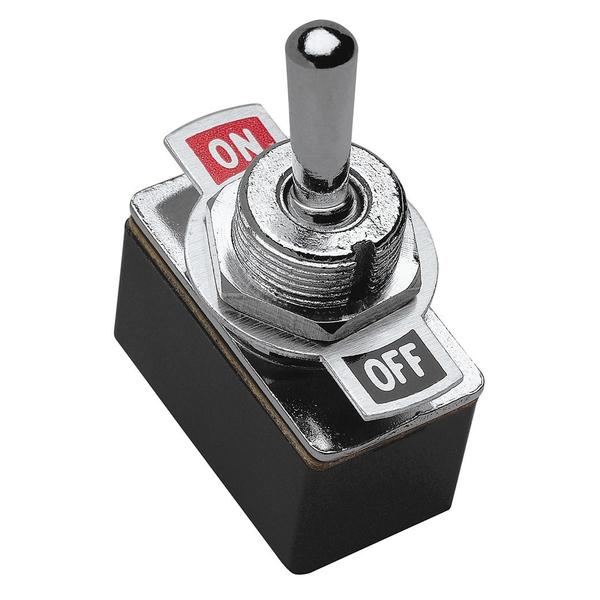
\includegraphics[scale=0.15]{figuras/eagle/toggle.png}
\caption{Interruptor de 2 posiciones}
\label{toggle}
\end{figure}

Estos interruptores ofrecen la funcionalidad que se necesita para un prototipo pero es necesario diseñar un dispositivo final para entregar al cliente. Es por esto nace el requerimiento de que se deba usar un botón único para encender y apagar el dispositivo y esto no es una tarea trivial.\\
	Los requerimientos para este botón es que baje a $0[V]$ cuando se apaga, que sea un único botón y que no requiere ninguna programación. \\

Un circuito muy utilizado que cumple los requerimientos anteriores se puede observar en la figura \ref{esquematico}.\\

\begin{figure}[H]
\centering
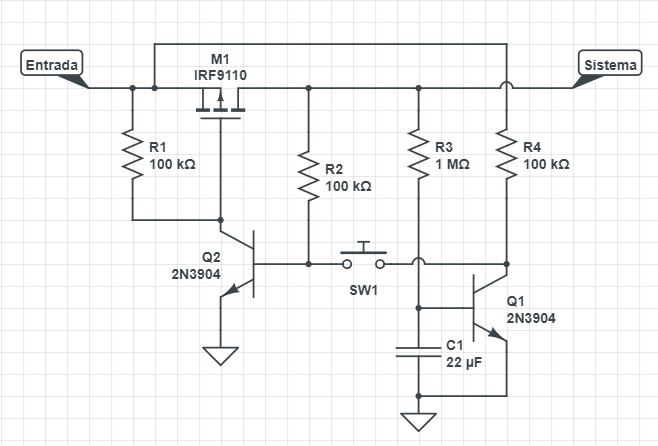
\includegraphics[scale=0.7]{figuras/eagle/circuito.png}
\caption{Circuito para botón ON/OFF}
\label{esquematico}
\end{figure}

Este circuito cumple con los requerimientos de ser simple, funcionar con un solo botón que cumple ambas funciones de encendido y apagado. \\
Alimentando el circuito con una entrada de $3[V]$ cuando se presiona el botón para encender, se alimenta la base del transistor Q2 lo que provoca que el mosfet M1 permita el paso de la corriente desde ''Drain'' hasta ''Source'' esto va a permitir que se alimente el sistema, además va a alimentar el transistor Q1 lo que va a permitir cargar el condensador C1.\\
El condensador C1 es utilizado para mantener alimentado el transistor Q1 ya que al presionar el botón, una persona normal podría demorar entre $0.1[s]$ a $0.5[s]$ en todo el proceso ya que es humano, por lo que se utiliza para cargarlo en ese tiempo y no se apague automáticamente al soltar el botón.\\
En una segunda etapa cuando se pulsa el botón para apagar, se corta la base del transistor Q2 y utilizando la resistencia equivalente del Arduino el condensador se va a descargar pasando la corriente hacia el sistema y finalmente se cortará la alimentación.\\
Probando este circuito con un osciloscopio se puede corroborar el funcionamiento de encendido y apagado como se muestra en la figura  \ref{on}

\begin{figure}[H]
\centering
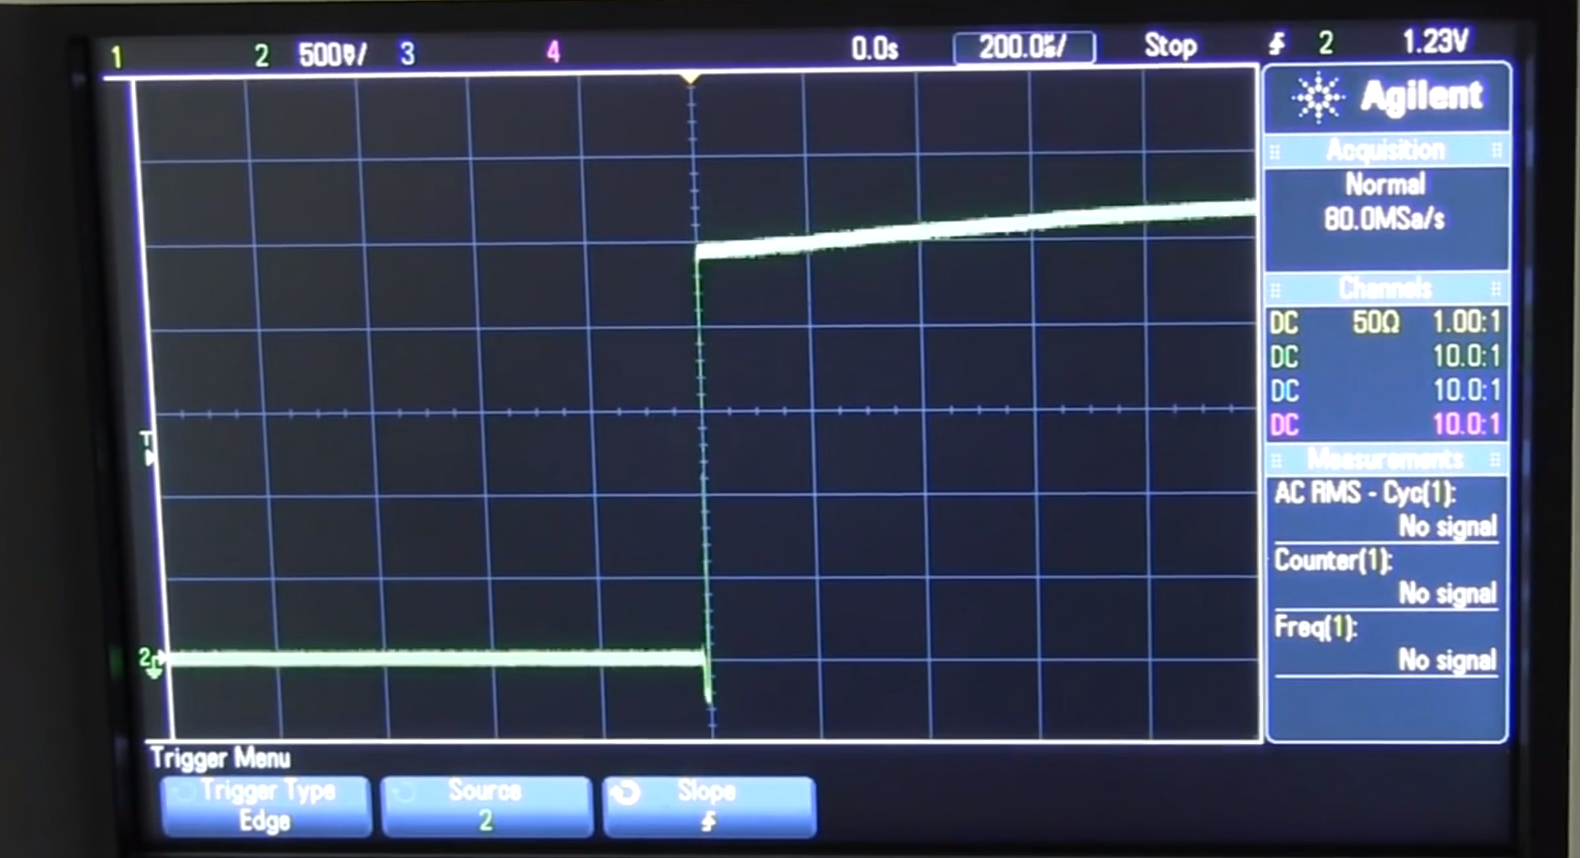
\includegraphics[scale=0.23]{figuras/eagle/on.png}
\caption{Función de encendido}
\label{on}
\end{figure}

Esto muestra lo poco que demora el circuito en pasar de un estado a otro y permite mantenerse encendido.

\begin{figure}[H]
\centering
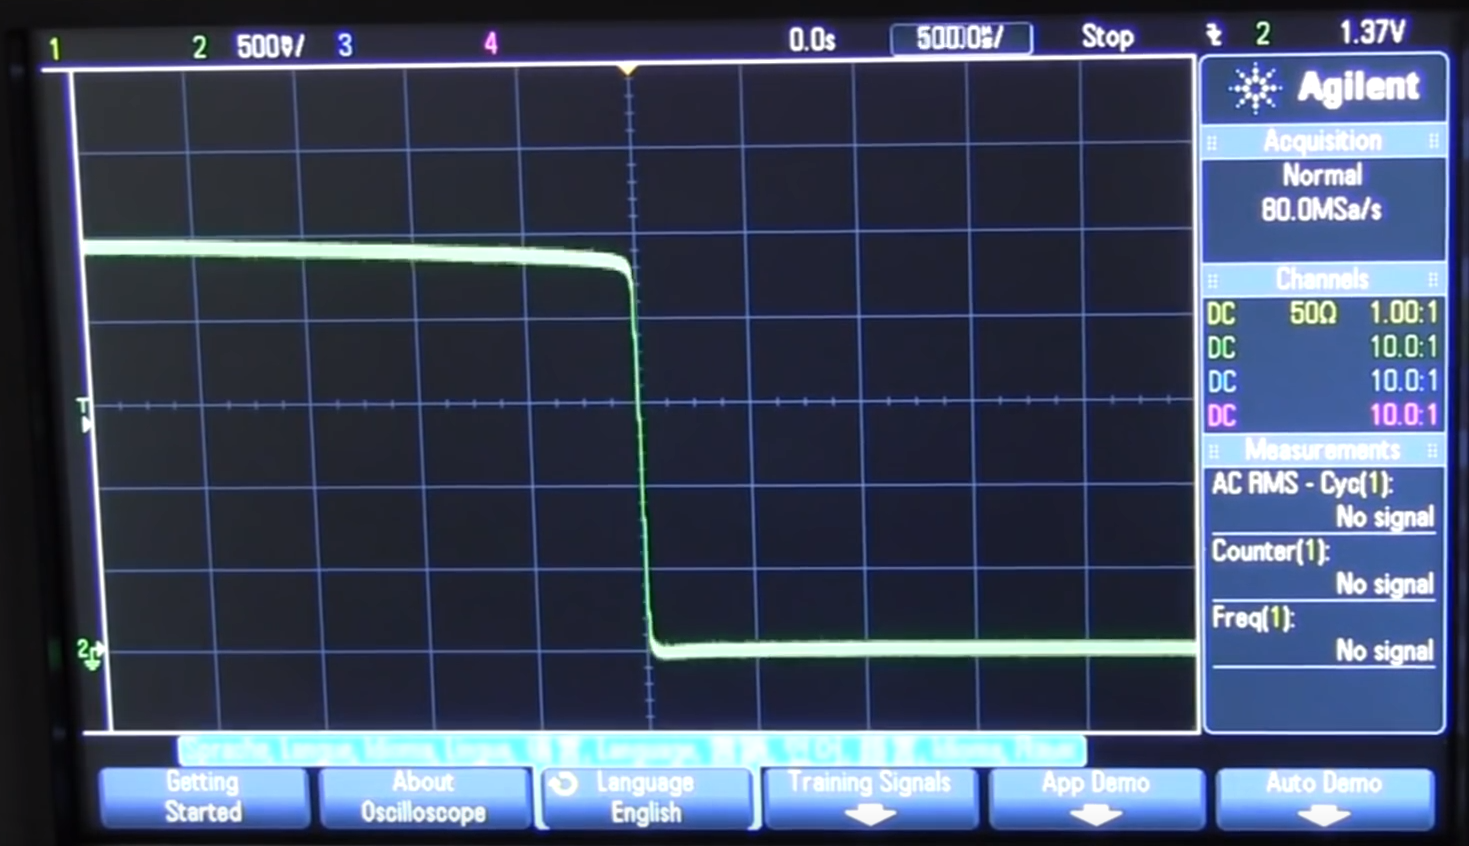
\includegraphics[scale=0.23]{figuras/eagle/off.png}
\caption{Función de apagado}
\label{off}
\end{figure}

En la figura \ref{off} se puede observar que también se demora poco tiempo en descargarse, debido a que está conectado a una carga muy grande y que pide mucha corriente, lo que hace que el tiempo de descarga del condensador C1 sea mucho menor. 

\section{Esquemático}
El diseño final dispositivo se puede considerar como 7 módulos en conjunto entre los cuales se encuentra el microcontrolador, ECG, cargador de batería, botón ON/OFF, FTDI, Bluetooth y regulador de voltaje los cuales resultan en un esquemático final que se puede observar en los anexos.\\
Los módulos mas grandes se explicaron en los capítulos anteriores, en esta sección se explicará el regulador de voltaje y los diseños finales para el dispositivo.
\subsection{Regulador de voltaje 3.3[V]}
Para proveer energía al microcontrolador y al sistema entero, es necesario un regulador de voltaje de bajo ruido que cumpla la función de evitar grandes variaciones que pueden provocar fallas en la PCB.\\
Todos los integrados utilizados tienen un rango aceptable de funcionamiento que varía entre los $2-5[V]$ aproximadamente. En este intervalo los valores comúnmente utilizados son $3.3[V]$ y $5[V]$.\\
La alimentación es un factor determinante a la hora de diseñar un microcontrolador ya que al utilizar un resonador para sincronizar su reloj, dependiendo del voltaje que se provee, este funciona a distintas velocidades como se puede observar en la figura \ref{atmega}.\\

\begin{figure}[H]
\centering
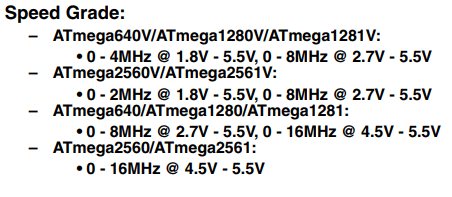
\includegraphics[scale=0.7]{figuras/eagle/atmega.png}
\caption{Velocidades y voltajes recomendados para un microcontrolador ATMega2560}
\label{atmega}
\end{figure}

Como se puede observar, es posible configurar el microcontrolador de $2[MHz]$ con voltaje entre $1.8[V]$ y $5.5[V]$. Además una velocidad de $8[MHz]$ se puede conseguir con un voltaje entre $2.7$ y $5.5[V]$. Finalmente se puede utilizar una velocidad de $16[MHz]$ con un voltaje entre $4.5[V]$ y $5.5[V]$.\\
Como una de las condiciones es que el dispositivo sea de pequeño tamaño y peso, se utilizará una batería de $4.3[V]$ de $950[mAh]$ y es por esto que se va a bajar la velocidad a $8[MHz]$ para utilizar una alimentación de $3.3[V]$.\\

Se utilizará un integrado MIC5219 el cual ofrece un regulador de bajo ruido que funciona a $3.3[V]$ y permitirá energizar el dispositivo. En la figura \ref{reg} se puede observar el integrado y su configuración típica.

\begin{figure}[H]
\centering
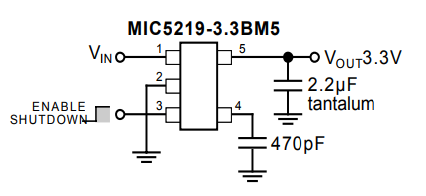
\includegraphics[scale=1]{figuras/eagle/reg.png}
\caption{Regulador de voltaje 3.3[V]}
\label{reg}
\end{figure}

Para entender este diagrama es necesario destacar $V_{in}$ que viene a ser la alimentación de la batería de Li-ion, $V_{out}$ es la salida de $3.3[V]$ hacia la carga que involucra el microcontrolador y todas las componentes del sistema.\\
El pin 2 es la tierra del sistema y el pin 3 ofrece una función para habilitar y deshabilitar el regulador la cual no se va a utilizar. Finalmente el pin 4 ofrece reducción de ruido conectandolo a tierra con un condensador de $470[pF]$.

\subsection{Conector para sensores}
Al trabajar con sensores, es necesario facilitar la tarea para el diseñador de producto de conectar las entradas al sistema con el vestible, es por esto que se va a reducir todos los sensores a un solo conector. Para esto, considerando que se utilizará el ECG y 2 sensores de temperatura para promediar su valor y obtener mayor precisión, se necesitan 5 conectores para los datos y además alimentación y tierra.\\

\begin{figure}[H]
\centering
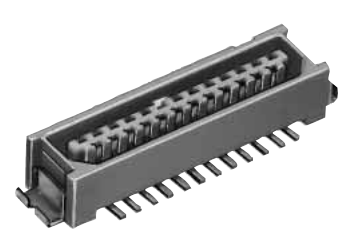
\includegraphics[scale=0.5]{figuras/eagle/conn.png}
\caption{Conector para sensores}
\label{conector}
\end{figure}

El conector que se utilizará se puede observar en la figura \ref{conector}. La particularidad que ofrecen estos tipos de conectores es que poseen entre 9 y 51 contactos.\\
Para el diseño se van utilizar 9 contactos los cuales constan de 3 conectores para los 3 electrodos de ECG, 2 para sensores de temperatura y 4 de alimentación (Voltaje y tierra para ECG independientes de la alimentación de los sensores de temperatura) como se puede observar en la figura \ref{coneagle}.

\begin{figure}[H]
\centering
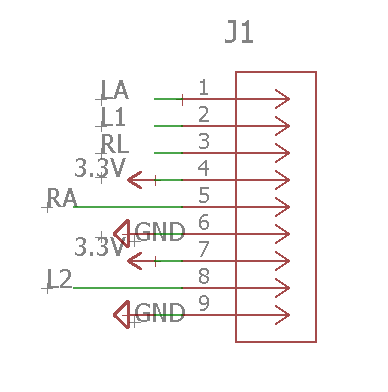
\includegraphics[scale=0.5]{figuras/eagle/sensores.png}
\caption{Conector de 9 pines}
\label{coneagle}
\end{figure}

\subsection{Pin header para prototipo}
Finalmente, como el microcontrolador ofrece 16 pines análogos, 54 digitales y 14 PWM se dejarán headers en la primera iteración del dispositivo para que se pueda seguir prototipando y agregar mas sensores en el futuro, donde se pueda trabajar en el mismo dispositivo en vez de utilizar uno independiente. \\
También se va a dejar disponible pines para comunicación UART (2 utilizadas en el dispositivo y 2 libres) y también los pines SDA y SCL para comunicación I2C. \\

\begin{figure}[H]
\centering
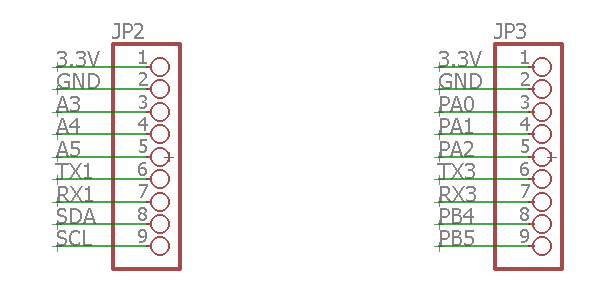
\includegraphics[scale=0.5]{figuras/eagle/header.png}
\caption{Conección Headers}
\label{header}
\end{figure}

Como se puede notar en la figura \ref{header} estos pines ofreceran alimentación y comunicación UART en cada header. 3 pines analogos (A3, A4 y A5), los 2 pines de conección I2C (SDA y SCL) y 5 pines digitales (PA0, PA1, PA2, PB4 y PB5).







%Capítulo 8: Configuración RN4020
\newpage
\chapter{Configuración RN4020}\label{rn4020}
%\newpage
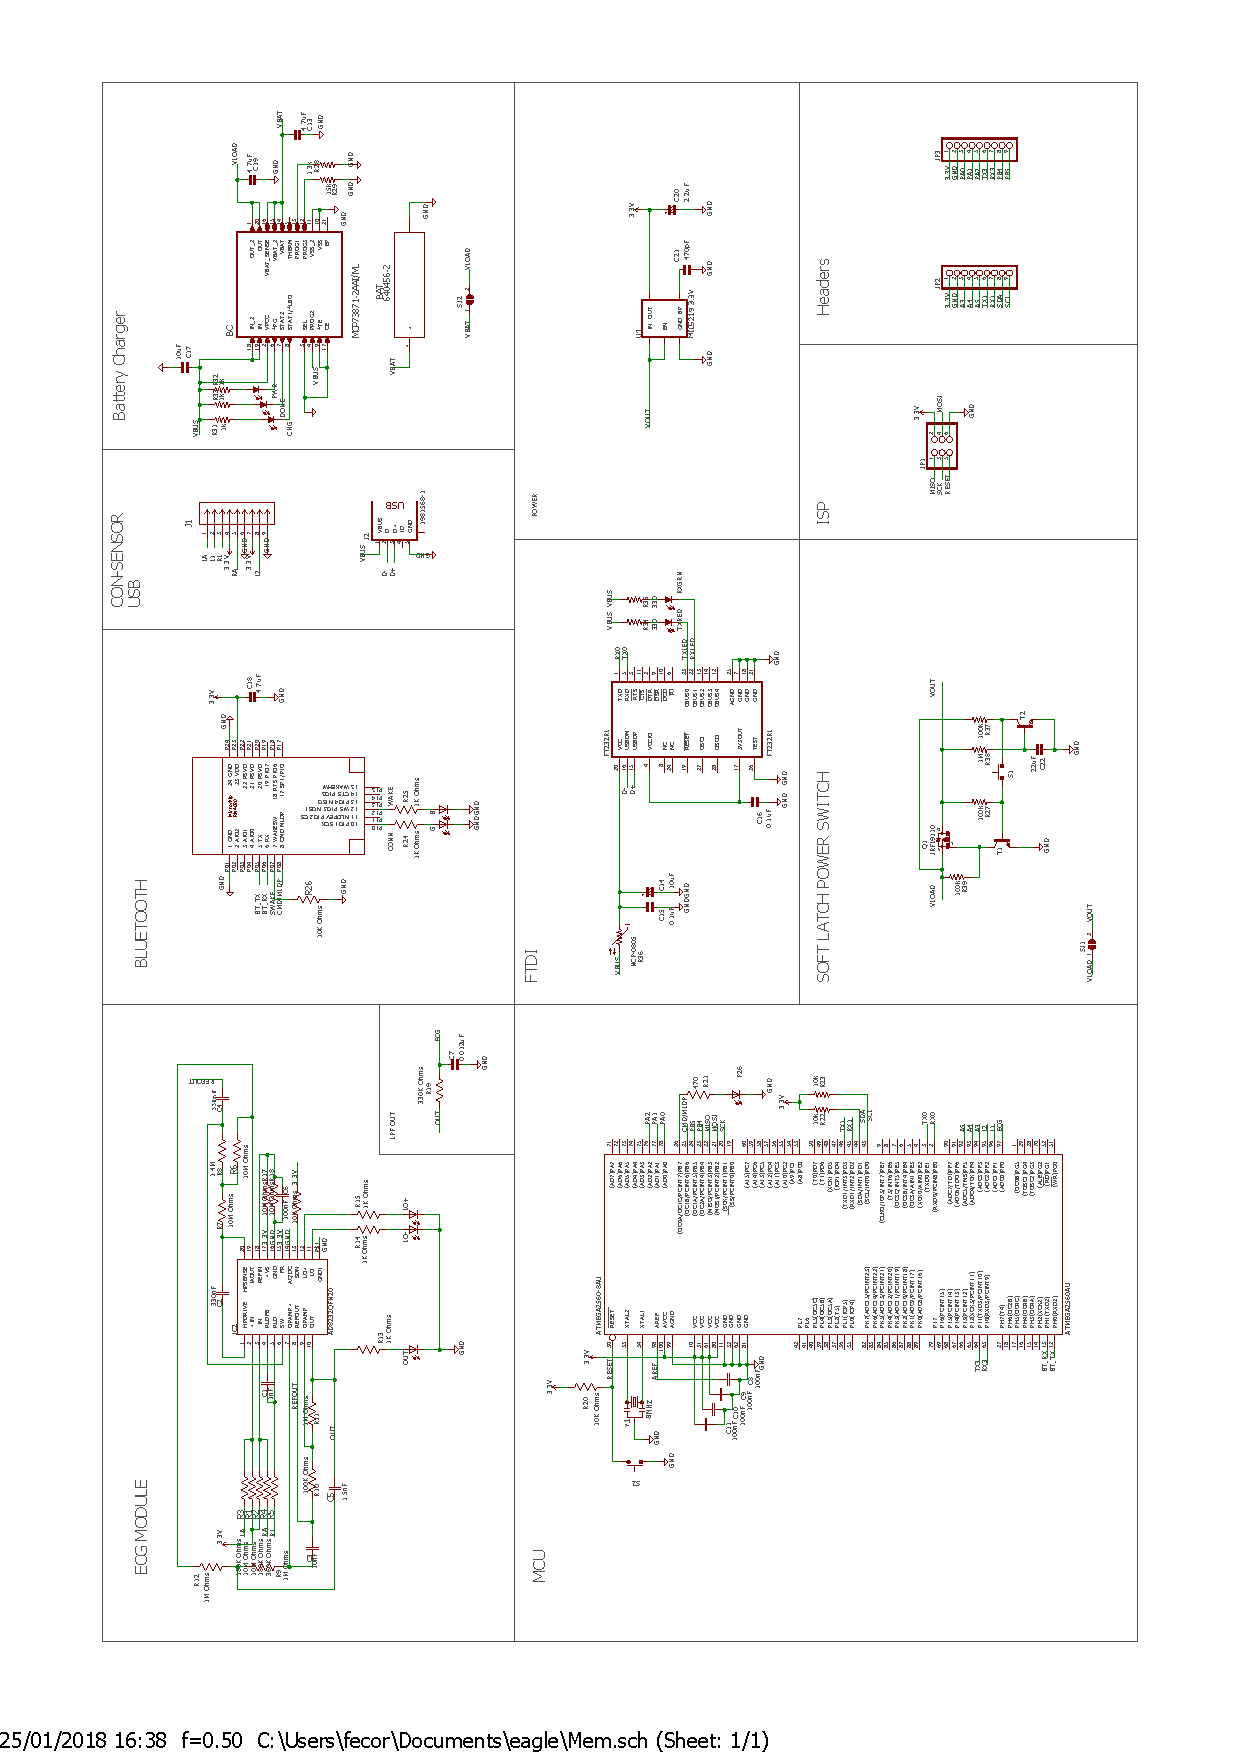
\includepdf[pages={-},scale=0.9,pagecommand={}]{figuras/anexos/esquematic.pdf}
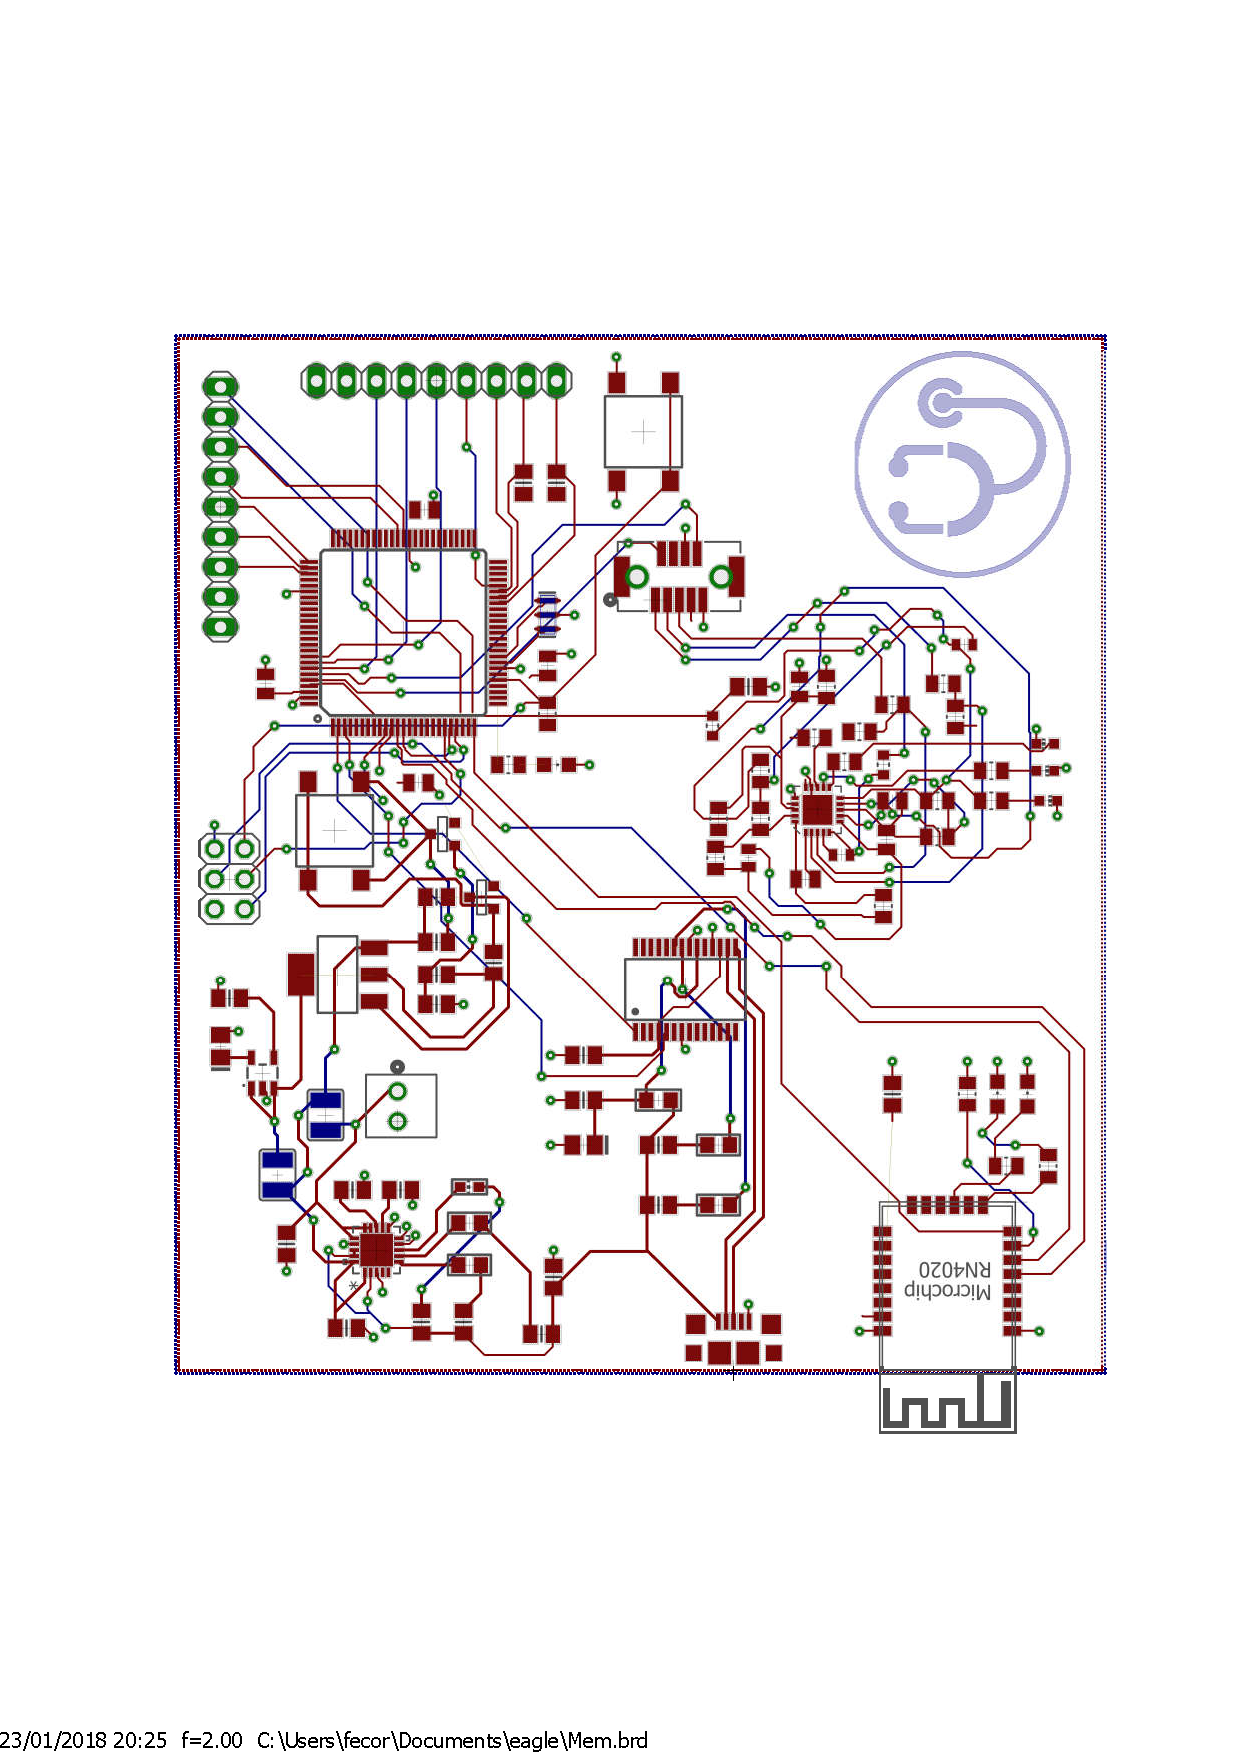
\includepdf[pages={-},scale=1.1,pagecommand={}]{figuras/anexos/board.pdf}
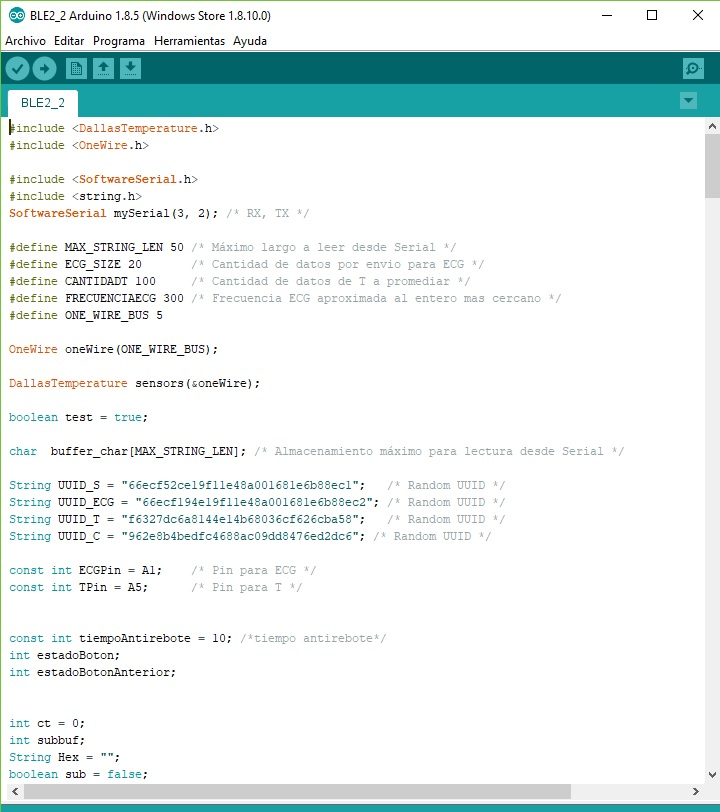
\includegraphics[width=1\textwidth]{figuras/anexos/code1.jpg}
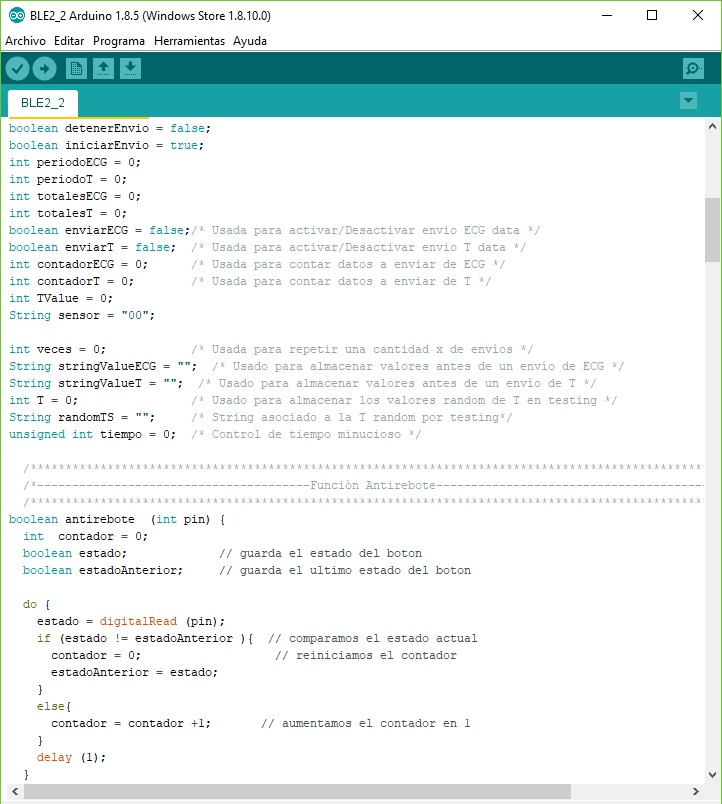
\includegraphics[width=1\textwidth]{figuras/anexos/code2.jpg}
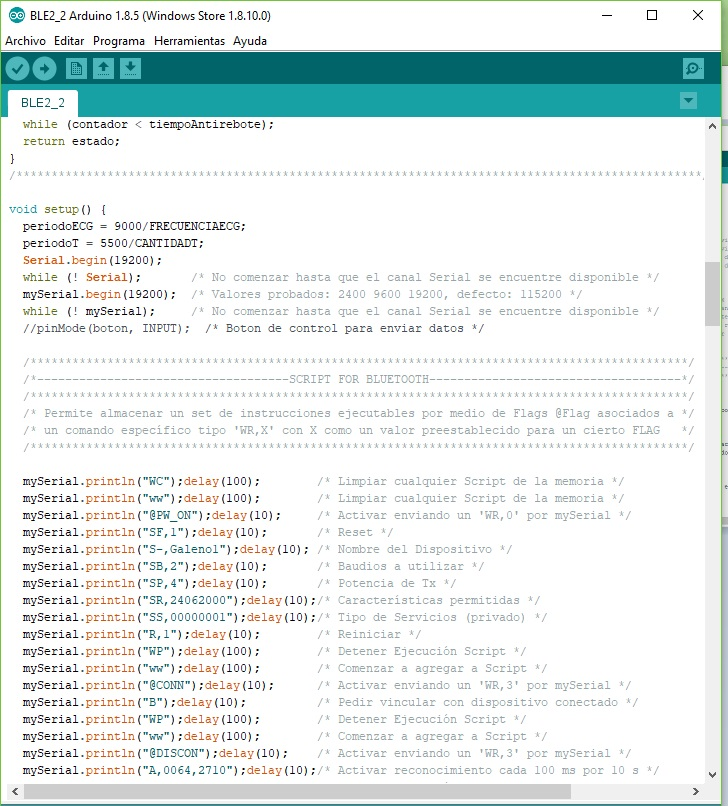
\includegraphics[width=1\textwidth]{figuras/anexos/code3.jpg}
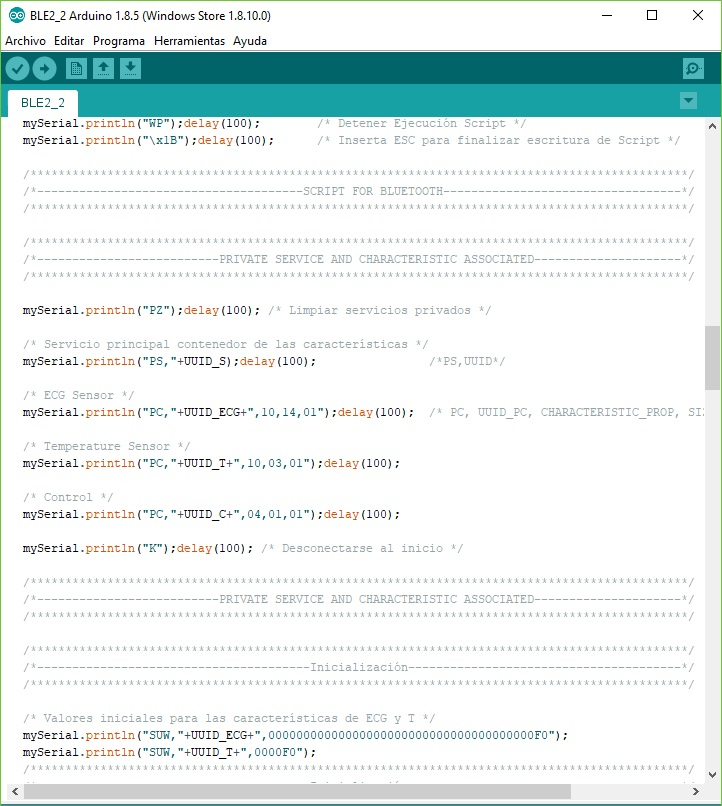
\includegraphics[width=1\textwidth]{figuras/anexos/code4.jpg}
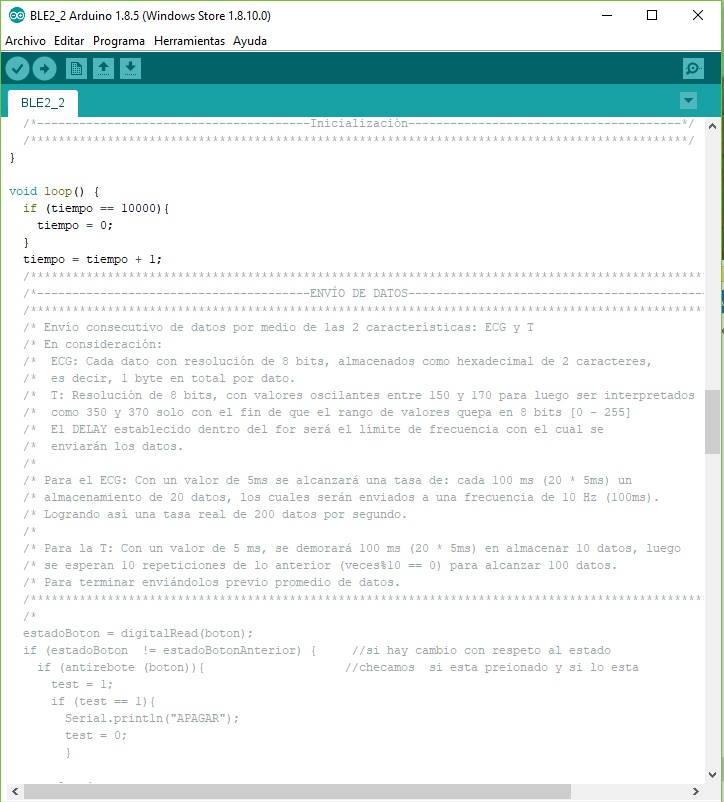
\includegraphics[width=1\textwidth]{figuras/anexos/code5.jpg}
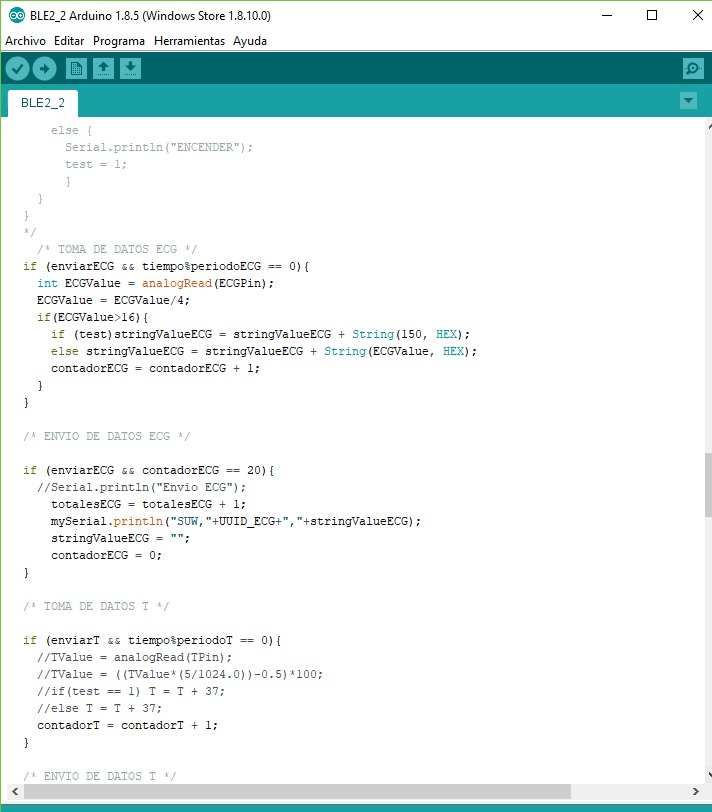
\includegraphics[width=1\textwidth]{figuras/anexos/code6.jpg}
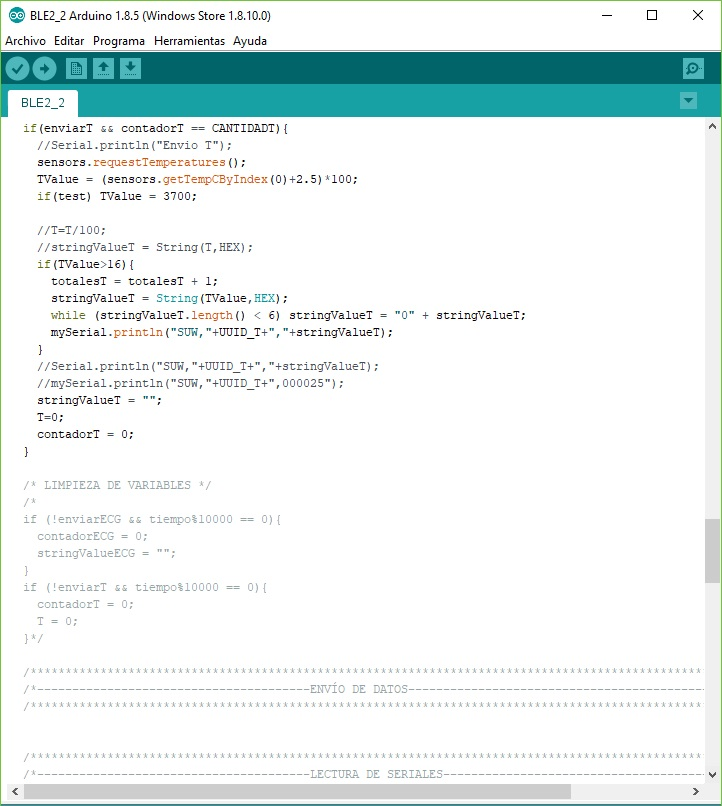
\includegraphics[width=1\textwidth]{figuras/anexos/code7.jpg}
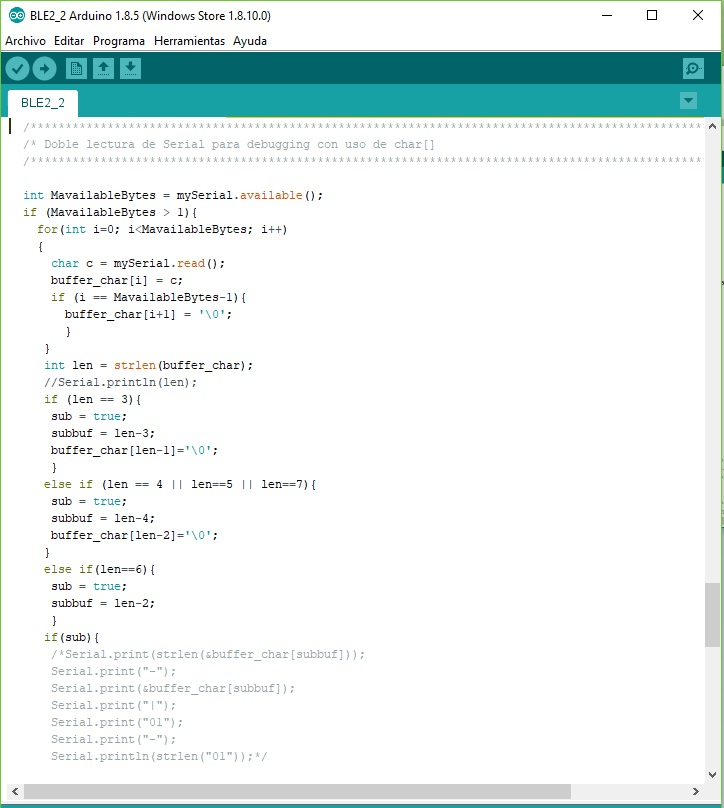
\includegraphics[width=1\textwidth]{figuras/anexos/code8.jpg}
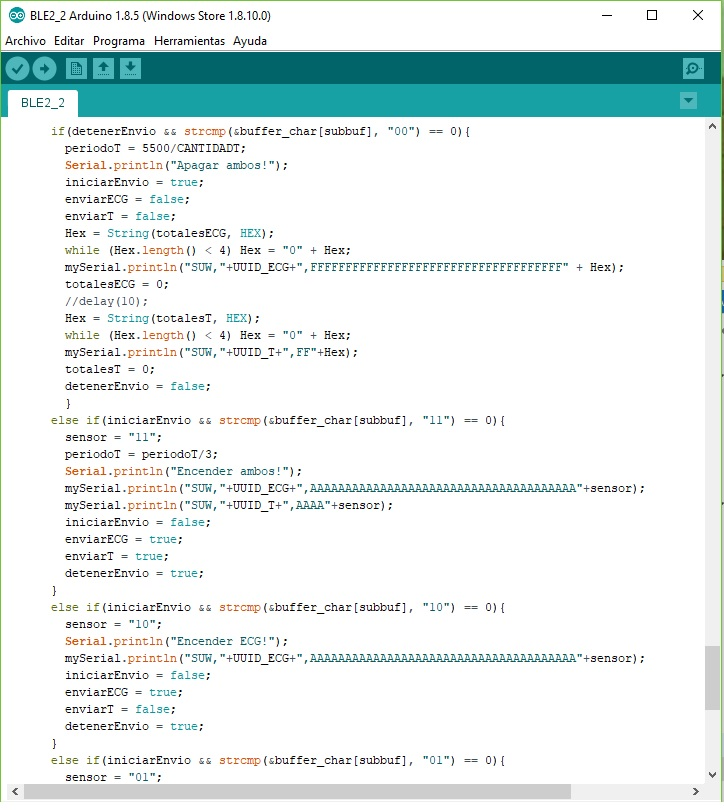
\includegraphics[width=1\textwidth]{figuras/anexos/code9.jpg}
\centering
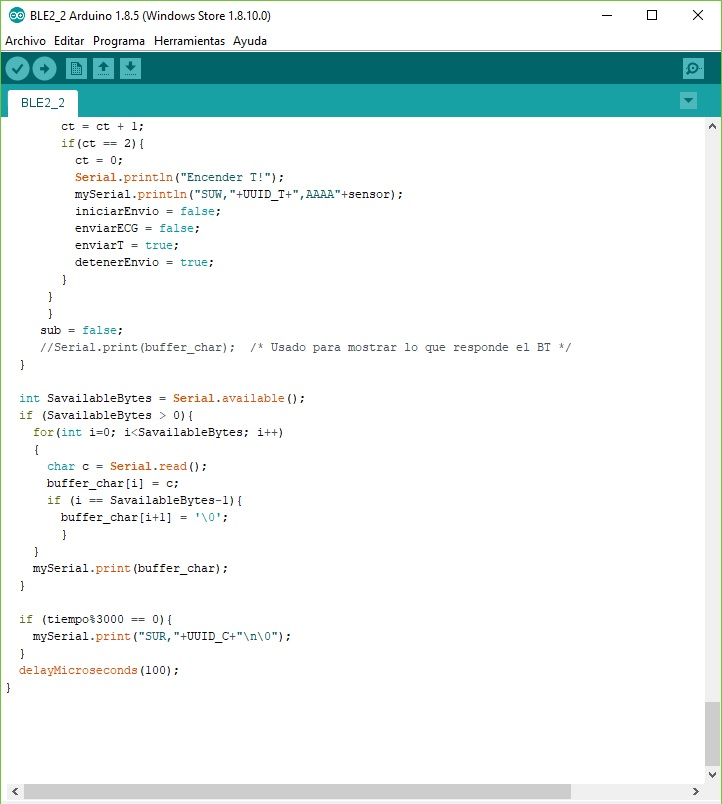
\includegraphics[width=1\textwidth]{figuras/anexos/code10.jpg}


%Capítulo 9: Integración de las componentes de la solución
\newpage
% ---------------------------------------------------------------------------------------
\chapter{Integración de las componentes de la solución}\label{mldp}
En esta sección se abordará el hardware utilizado para prototipado y diseño de bluetooth bajo consumo (BLE - bluetooth low energy). 

\section{BLEBee}
Para el prototipado se utilizará un módulo bluetooth BLEBee que ofrece una conexión simple a placas Arduino que posean este puerto. 
BLEBee utiliza un módulo de bluetooth RN4020 el cual ofrece bluetooth versión 4.1.\\
Mediante interfaz UART, este modulo puede ser configurado para actuar como módulo central o periférico cuando establezca una conexión.\\
Para conocer mas el funcionamiento de este módulo primero hay que conocer mejor la conexión XBee.

\begin{figure}[H]
\centering
\includegraphics[scale=1]{figuras/bluetooth/xbee.png}
\caption{Forma y Pines de puerto XBee}
\label{xbee}
\end{figure}

Como se puede observar en la figura \ref{xbee} el puerto XBee ofrece una conexión de 20 pines con usos generales que se utilizan por distintos dispositivos, en este caso bluetooth.\\
En el caso de BLEBee la distribución de los pines se puede observar en la figura \ref{blebee}

\begin{figure}[H]
\centering
\includegraphics[scale=0.5]{figuras/bluetooth/blebee.png}
\caption{Distribución de pines BLEBee}
\label{blebee}
\end{figure}

Comparando la figura \ref{xbee} con la figura \ref{blebee} se puede observar los pines mas relevantes a la hora de diseñar un módulo bluetooth en el dispositivo, siendo los pines mas importantes, y contrastando con el datasheet, los que se muestran en la tabla \ref{pines}

\begin{table}[H]
\centering
\begin{tabular}{| c | c | c |}
\hline
\multicolumn{1}{|c|}{\textbf{Nº Pin}}&
\multicolumn{1}{c|}{\textbf{Nombre}}&
\multicolumn{1}{|c|}{\textbf{Descripción}}\\ \hline
5  & UART TX & Transmisor UART\\ \hline
6  & UART RX & Receptor UART\\ \hline
7  & WAKE\_ SW & Despertador de modo deep sleep\\ \hline
10 & Led Conexión  & Led indicador de conexión\\ \hline
12 & Led Actividad & Led indicador de actividad\\ \hline
\end{tabular}
\caption{Pines relevantes módulo RN4020}
\label{pines}
\end{table}

\newpage
\section{Comunicación UART}

La comunicación UART (Universal Asynchronous Receiver-Transmitter) es un formato de comunicación serial donde el formato y la velocidad de transmisión son configurables. Un UART puede ser un circuito integrado independiente pero en la actualidad vienen incluidos en los microcontroladores.\\
Para entender mejor como funciona la comunicación serial mediante UART hay que observar la figura \ref{UART}

\begin{figure}[H]
\centering
\includegraphics[scale=0.8]{figuras/bluetooth/uart.png}
\caption{Configuración para comunicación UART}
\label{UART}
\end{figure}

La comunicación UART cuenta de 2 pines TX (transmisor) y RX (receptor) el cual se conecta al Receptor y transmisor del microcontrolador respectivamente.

\section{Diseño del módulo bluetooth}
Finalmente contrastando lo visto anteriormente y con referente a la tabla \ref{pines} se puede diseñar el esquemático del integrado.\\
Pin 5 y 6 corresponden a la comunicación UART como se explica en la figura \ref{UART}. Es necesario conectar los pines 10 y 12 con diodos led ya que son pines indicadores, el pin 10 indica el estado de la conexión con un led verde y también se recomienda conectar un led azul al pin 12 para ver el estado de actividad (ej. Si se está enviando información o está dormido).\\
El pin 7 cumple la función de despertar el módulo bluetooth cuando se encuentre dormido emitiendo desde el microcontrolador una señal de $3.3[V]$.\\
\begin{figure}[H]
\centering
\includegraphics[scale=0.8]{figuras/bluetooth/eagle.png}
\caption{Esquemático bluetooth diseñado en EagleCAD}
\label{eagle}
\end{figure}

Como se puede observar en la figura \ref{eagle} se conecta el módulo bluetooth con los pines descritos. Se utiliza un condensador en la alimentación de módulo para regular el voltaje de la entrada.






%Capítulo 10: Prototipo funcional V1
\newpage
% ---------------------------------------------------------------------------------------
\chapter{Prototipo funcional V1}\label{proto1}
Al ver el esquemático terminado y las piezas seleccionadas se puede notar que se cumplen los requisitos propuestos en un principio. Realizando un listado de costos de componentes se obtiene un valor de $42 USD$ total. Además el costo de fabricación de una PCB de tamaño menor a $10x10[cms]$ es de aproximadamente $7 USD$. Lo que lleva a un costo total del dispositivo de $49 USD$ contando solamente componentes electrónicas.\\
Es importante destacar que esta primera versión del dispositivo es solo un comienzo en la larga etapa de desarrollo, luego de producir esta primera placa se debe realizar las pruebas correspondientes y verificación de integridad de la placa.\\
El diseño final de la PCB se puede observar en los anexos.\\
Además se aprendió a diseñar un dispositivo electrónico desde su prototipo en una placa de desarrollo, donde fue necesario leer constantemente las hojas de datos de todas las componentes a utilizar y seleccionar cuales son las mejores, que al mismo tiempo sean compatibles y coherente con el diseño que se está llevando a cabo.\\
También es importante destacar la experiencia que se obtuvo con el concurso de emprendimiento. Se aprendió mucho del mundo del emprendimiento al presentar el trabajo realizado. Además se tuvo la oportunidad de observar los trabajos propuestos por los otros emprendedores y estudiar los criterios de evaluación. Se dió mucha importancia al modelo de negocios y las alianzas estratégicas que tenía cada participante, mas que al trabajo realizado y estado actual de la idea o prototipo. Muchos de los seleccionados ya tenían potenciales clientes y alianzas estratégicas que los hacía mejores candidatos a ganar el dinero para el emprendimiento.

%Capítulo 11: Prototipo funcional V2
\newpage
\chapter{Prototipo funcional V2}\label{proto2}

Este trabajo tuvo el propósito de buscar una solución al desafío propuesto por la empresa Sistemas Expertos. Como grupo multidisciplinario se tomó la decisión de no dejar el trabajo e investigación realizada solo como un prototipo por lo que se llevó al área del emprendimiento postulando a fondos para desarrollar mejor la idea y proponer el modelo de negocios desarrollado durante el año.

\section{Transformación de memoria multidisciplinaria a emprendimiento}
Al finalizar el diseño del dispositivo y tener un prototipo funcional como grupo de memorias multidisciplinarias se decidió continuar trabajando en el desafío con una alianza estratégica con la empresa Sistemas Expertos.\\
Se realizaron entrevistas con profesionales de la salud en el área de Quintero y se postuló a un torneo de emprendimiento del instituto 3IE de la universidad Santa María.\\
El Instituto 3IE tiene como principal objetivo apoyar el desarrollo y aceleración de emprendimientos de base tecnológica, con mérito innovador y alto potencial de escalamiento, a través de su Programa de Incubación, cuya principal propuesta de valor se basa en vinculación temprana con el sector productivo o empresarial, la validación técnico y comercial de las soluciones (productos y/o servicios), la gestión comercial, y el financiamiento temprano para hacer despegar los negocios.\\
Este Programa, se implementa bajo la línea de financiamiento Torneos de Emprendimiento Tecnológico, apoyado por CORFO y ejecutado por el Instituto 3IE, y que busca instalar capacidades y conocimientos en tecnologías habilitantes para el desarrollo de nuevas soluciones tecnológicas que logren un impacto positivo en la competitividad y eficiencia del sector industrial o público.\\

\begin{figure}[H]
\centering
\includegraphics[scale=0.3]{figuras/chamullo/corfo.jpg}
\caption{Desafío IoT propuesto por el instituto 3IE}
\label{3ie}
\end{figure}

\newpage
Este concurso posee una planificación del proceso completo que se puede observar en la figura \ref{proceso}

\begin{figure}[H]
\centering
\includegraphics[scale=0.85]{figuras/chamullo/proceso.jpg}
\caption{Planificación desafío IoT}
\label{proceso}
\end{figure}


\subsection{Entrevista a doctores en hospital de Quintero}
Se realizaron entrevistas a 2 profesionales de la salud en el hospital de quintero para evaluar la factibilidad del emprendimiento y ver el problema desde el punto de vista de quienes trabajan en el sector público.\\
Primero se realizó la entrevista a Fabián Álvarez, medico general de zona y cuyo cargo es jefe de urgencia. También se realizó una entrevista al doctor Cristian Mondaca, Jefe del programa de salud cardiovascular y jefe de farmacia. 
\subsubsection{Entrevista a Fabián Álvarez}
En la entrevista comenta que los adultos sanos realizan controles 1 vez al año y se hacen exámenes preventivos. Además existe un programa de salud cardiovascular para personas mayores de 18 años, según guías clínicas "Enfoque de riesgo cardiovascular" del MINSAL (2015), cada 3, 6 y 12 meses en los cuales se hacen exámenes de laboratorio, electrocardiograma, se mide presión arterial, peso y estatura. 
Los problemas que se identificaron fueron la poca disponibilidad de exámenes y recursos humanos para atender a la demanda programada. Además implementan telemedicina por medio de fotos para dermatología donde le envían estas a algún especialista, teleasistencia broncopulmonar mediante videoconferencia y teleasistencia para electrocardiograma el cual intenta no usarse demasiado.\\
Debido a la sobre demanda del sistema de urgencias, los profesionales de la salud deciden hacer una categorización de pacientes desde C1 a C5 donde C5 significa que requiere asistencia inmediata y C1 puede ser que el paciente vuelva otro día.\\
Finalmente se hizo una encuesta donde el médico debía dar un valor a las siguientes afirmaciones según un ranking de dolor entre 1 y 10 como se muestra en la tabla \ref{fabian}
\newpage
\begin{table}[H]
\centering
\begin{tabular}{| c | c |}
\hline
\multicolumn{1}{|c|}{\textbf{Afirmación}}&
\multicolumn{1}{|c|}{\textbf{Nota de Dolor}}\\ \hline
Muchos Recursos por IIH  & 3-4  \\ \hline
Necesidad de control mas rápido en urgencias & 8 \\ \hline
Reclamo por el servicio  & 10  \\ \hline
Reclamos internos de los médicos & 10\\ \hline
Bajos recursos para mejorar atención & 10\\ \hline
\end{tabular}
\caption{Ranking de dolor Fabián Álvarez}
\label{fabian}
\end{table}

\subsubsection{Entrevista a Cristian Mondaca}
Como jefe del programa de salud cardiovascular, da énfasis en el riesgo cardiovascular con controles cada 3, 6 y 12 meses y destaca que muchas veces se atrasa a los pacientes que van mejorando pese a que no se debería hacer debido a la disponibilidad de horas médicas y la cantidad de pacientes.
En caso de mayor necesidad se tiene contemplado el uso de una hora extra al mes siguiente por exámenes nuevos.\\
Se mostró un vídeo con el prototipo funcional realizado en este trabajo de tesis y el médico hace la observación de que para realizar controles se requiere hacer un ECG completo, es decir, se necesitan las 6 precordiales y las 3 tradicionales (2 electrodos en brazos y 1 en pierna). \\
En la entrevista destaca que para realizar pruebas en pacientes reales se debe hablar con el director del hospital y desarrollar un consentimiento informado de parte del paciente. \\
Un dato importante que resalta es la cantidad de pacientes en el programa de salud cardiovascular el cual alcanza un total de 1900 incluyendo hipertiroidismo, de los cuales 1500 son de mayor riesgo.\\
Entre las ideas propuestas por el médico se destaca la necesidad de tener una base de datos con historial de electrocardiogramas ya que al realizar exámenes tradicionales estos se imprimen en un papel milimétrico y son otorgados a los pacientes, los cuales generalmente pierden esta información para la próxima consulta lo que hace más difícil un diagnostico preciso.\\
Finalmente se hace énfasis en que el hospital de Quintero es un hospital de baja complejidad y no hay especialistas, por lo que cuando hay alguna anormalidad se deriva a un cardiólogo o medico internista para realizar un informe y diagnosticar.\\
Cuando ocurre un infarto, es enviado en ambulancia directo a Viña del mar para que sea atendido por un especialista.

\subsection{Pitch day selecconados - Marzo 2018}
Para realizar el Pitch para el concurso se utilizó lo aprendido en los módulos de memoria y las clases impartidas por el desafío del instituto 3IE en los cuales dividen el pitch en 3 partes.\\
La primera parte es hablar del dolor, identificar cuantos tipos de cliente se ven afectados y mostrarlos en términos objetivos (cifras), con esto se debe presentar cuales son los analgésicos internos, externos y como se evitan este dolor y finalmente presentar una promesa de valor en la cual se explica, de manera simple, que logra nuestra solución. Para esto se recopiló información y se identificó que solo para el año 2016 fallecieron alrededor de $25.000$ personas esperando atención médica en alguno de los 203 hospitales públicos chilenos. De esos, $18.423$ ( $74\%$ aproximadamente) corresponden a personas sobre 65 años. Esto solo refleja un universo mucho mayor, cercano a $1.661.826$ de personas que estuvieron en lista de espera y la única forma de mitigar esto es por medio de categorización de pacientes por su nivel de riesgo, lo cual no disminuye las listas, sino que da prioridad a aquellos mas urgentes\\
La segunda parte consiste en el servicio propiamente tal, donde se plantea reducir las listas de espera y tener una gestión eficiente del capital humano donde los profesionales atienden donde y a quien corresponde en base a un historial. Proyecto Galeno ofrece una polera inteligente con sensores de electrocardiograma y temperatura conectada a un dispositivo Android que a su vez envía la información a un sitio web donde muestra en tiempo real la información y donde también se puede controlar el comportamiento del ecosistema.\\
En la tercera parte se muestra el plan de vuelo donde se dan a conocer los hitos relevantes del proyecto, el plan de negocio y el equipo. La obtención de dinero es posible a través de un sistema de arriendo mensual de los dispositivos y la plataforma en cada hospital, según las necesidades de cada uno. Como en caso concreto se tiene al Hospital de Quintero con alrededor de 34 camas disponibles y un ejemplo de pacientes con patologías cardiovasculares, pudiendo proyectar al menos entre $2000$ y $6000$ USD mensuales (considerando entre 10 y 30 dispositivos a $200$ USD cada uno).\\
Finalmente se cierra presentando el equipo y presentando nuestro aliado estratégico Sistemas Expertos, empresa que posee presencia en el mercado de la atención pública con 17 centros asistenciales a lo largo de Chile en el servicio de software para digitalización de la información.\\
En esta fase concluye la participación de Proyecto Galeno en el desafío IoT debido a que el jurado considera que la inversión en el desarrollo y la validación del dispositivo para obtener la certificación de grado médico es muy grande, se propone abordar este mismo problema externalizando el desarrollo con un dispositivo que ya tenga validación médica buscando aliados estratégicos para poder desarrollar a partir de esto. Además la presencia de Accuhealth en el mercado ofrece el mismo servicio con una mayor gama de sensores a un precio un poco superior al calculado por este proyecto, lo que hace muy difícil entrar al mercado de la salud privada y no consideran que entrar en el sistema de salud público sea una buena oportunidad.
\newpage
\section{Tareas Futuras}

La primera versión de un dispositivo electrónico es solo el comienzo de un largo camino en el desarrollo ya que es donde se puede evaluar de mejor manera el funcionamiento del diseño y evaluar cuales son los puntos a mejorar o cambiar. \\
En primera instancia se desea integrar la IMU en la siguiente iteración utilizando los headers de comunicación I2C que se diseñaron para prototipado y evaluar la posibilidad de cambiar el integrado amplificador para la señal del ECG a uno con menor ruido y mayor precisión. \\
Además se diseñó un modulo de botón ON/OFF y cargador de batería de forma independiente, lo cual se puede sustituir por un solo integrado lo cual disminuiría mucho el tamaño, pero esta idea fue descartada para la primera versión debido a que aumenta mucho el costo de fabricación debido a su empaquetado lo cual requiere un servicio adicional para soldarlo en la PCB final.\\


%Capítulo 12: Prototipo final
\newpage
\chapter{Prototipo final}\label{protof}
En el presente capítulo se ahondará en las distintas alternativas de diseño que existen para el prototipo con los distintos sensores requeridos, además de establecer la comunicación y el envío de la información tomada del paciente. Las etapas para el desarrollo del prototipo constan de: Elección de sistema de procesamiento o unidad central, sensores a utilizar y forma de comunicación inalámbrica.
\section{Plataforma de desarrollo}\label{proce}
Al fabricar un prototipo, el desarrollador debe construir el hardware sobre el cual correrá el software del producto que ha diseñado, por lo que debe tomar componentes de diversos proveedores, integrarlos y hacerlos funcionar como un conjunto. Por esa razón se popularizó el uso de plataformas de desarrollo electrónico.  \\
Por lo general, estas son placas que integran microcontroladores, circuitos y componentes electrónicos que le proporcionan diversas capacidades básicas y a partir de esto se puede evaluar la compatibilidad del diseño tanto en hardware como en software antes de enviar a fabricar el producto final. 

\newpage
\subsection{Arduino}
Arduino es una plataforma de desarrollo de bajo costo que permite crear proyectos de base tecnológica de forma sencilla y barata, que consta de entradas análogas, entradas y salidas digitales, PWM, comunicación serial, etc. 

Uno de los beneficios de Arduino es que provee módulos de desarrollo de bajo costo para trabajar con integrados y estudiar su funcionamiento y prototipado.
Arduino trabaja con una gran variedad microcontroladores AVR que diferencia por modelos dependiendo de las necesidades de proyecto, motivo por el cual varía en precio. 

En primera instancia se puede trabajar con un modelo Arduino UNO que es de bajo costo y permite leer señales análogas y traducirlas en su conversor análogo-digital y dependiendo de las necesidades se puede conseguir otro modelo como Arduino Mega que ofrece mayores prestaciones. 
\subsection{Raspberry}
Raspberry es una computadora de placa reducida (SBC por sus siglas en inglés) de bajo costo, con el objetivo de estimular la enseñanza de ciencias de la computación, no obstante, es de propiedad registrada para poder mantener el control de la 8 plataforma y no se generan excesivas variantes como es el caso de Arduino. El software que usa es open source, aunque es capaz de ejecutar incluso una versión de Windows 10. Por lo mismo su capacidad de procesar señales es mayor y permite ejecutar proyectos más complejos. No se define si es que pueden o no ser usadas en desarrollos comerciales.

\newpage
\subsection{Beaglebone}
Beaglebone black es la última iteración de la serie Beaglebone y su versión pequeña. Esencialmente es similar a Raspberry, diferenciándose en cosas como la capacidad para iniciarse sin la necesidad de instalar ningún sistema operativo ya que tiene memoria integrada, no así Raspberry. Adicionalmente cuenta con una cantidad de entradas sustancialmente mayor, por lo que permite hasta el doble de conexiones que su competencia directa. Como si es no fuera suficiente, la arquitectura del procesador que incluye Beaglebone black permite que rinda hasta el doble de rápido que su contraparte en Raspberry pi. \\
Al igual que su competencia, Beaglebone ofrece mucho mas procesamiento que el necesario por lo que se descarta como una opción para el desarrollo inicial del prototipo, de acuerdo a las necesidades que vayan surgiendo se puede considerar nuevamente como una opción.
\newpage
\section{Sensores}
Hablando con la contraparte de Sistemas Expertos se decidió, a partir de la información que proveen ellos, que las enfermedades  mas comunes son las afecciones cardíacas y también es necesario tener un control de la temperatura de los pacientes a la hora de leer sus signos vitales. \\
Por otra parte se propuso utilizar una IMU para detectar si algún paciente sufre una caída, este con el fin de emitir una alarma para llamar una ambulancia en caso de ser necesario.
\subsection{ECG}
Electrocardiograma o ECG es el proceso de registrar la actividad eléctrica del corazón en un periodo de tiempo usando electrodos directamente en la piel.\\
Lo fundamental será buscar un circuito de desarrollo para realizar una prueba de concepto, en la cual se puedan tomar los datos y manejar.
\subsubsection{DFRobot Heart Rate Monitor Sensor}
El monitor de actividad cardiaca de la empresa DFRobot se usa para medir la actividad electrica del corazón con un integrado AD8232\cite{ad8232} que toma señales análogas de los electrodos y utiliza amplificadores para tener una mejor lectura de los datos.\\
Utilizando un Arduino es posible leer los datos tomados de los electrodos y convertirlos a información digital que puede ser enviada por comunicación serial.\\

\begin{figure}[H]
\centering
\includegraphics[scale=0.5]{figuras/sensor/ecg/ecg.png}
\caption{Placa de desarrollo ECG}
\label{ecg}
\end{figure}

Como se puede observar en la figura \ref{ecg} posee conexión simple para electrodos y salida análoga, lo que permitirá una rápida prueba de concepto para utilizar este integrado en el diseño del dispositivo final. Además este provee filtros que se van a estudiar mas adelante.


\subsubsection{ADS1298}
El integrado ADS1298 de la empresa Texas Instrument ofrece un ECG con 8 amplificadores programables de bajo ruido y 8 conversores Análogo-digital de alta resolución.\\
Utilizado para instrumentación medica y lectura tanto de ECG como EMG (Electromiograma) y EEG (Electroencefalograma).\\
El integrado ADS1298 es una buena opción para un desarrollo de ECG en el futuro de grado médico, pero es de un precio 10 veces mayor al dispositivo de DFRobot por lo que se va a descartar para el prototipo funcional.
\subsection{Temperatura}
Cuando se requiere realizar alguna medición a un paciente siempre es necesario conocer su temperatura corporal que sirve como información complementaria a los profesionales de la salud es por esto que se evaluarán termistores que permitan la lectura de este dato.
\subsubsection{Lilypad Temperature Sensor}
Dentro de la tendencia del hardware abierto, uno de los proyectos más destacados es Lilypad Arduino, un conjunto de piezas electrónicas que se pueden coser a los tejidos para darles interactividad con sensores, luces o sonidos.\\
Entre estos sensores tenemos un sensor de temperatura compuesto por un termistor MCP9700 el cual ofrece una resolución de $\pm2^\circ C.$\\

\newpage
La particularidades que ofrece este sensor es ser de muy bajo costo y a su vez es impermeable por lo que permitiría incorporarlo en el wearable de forma permanente sin dañar la componente.

\begin{figure}[H]
\centering
\includegraphics[scale=0.7]{figuras/sensor/t/lilypad.jpg}
\caption{Sensor de temperatura Lilypad}
\label{Lilypad}
\end{figure}

Como se puede observar en la figura \ref{Lilypad}, Lilypad ofrece una PCB impermeable con 3 terminales que permiten utilizar un hilo conductor para coser este a la ropa.

\subsubsection{DS18B20}
El sensor DS18B20\cite{temp} es un termómetro digital que ofrece una medida de 9 a 12 bits de resolución. Se comunica mediante el bus 1-Wire (protocolo de comunicación en serie diseñado por Dallas Semiconductor el cual está basado en un maestro y varios esclavos en una sola linea de datos) lo cual permitiría, en caso de ser necesario, incorporar mas sensores para obtener una medida con mayor precisión. 
Este termómetro digital ofrece una resolución de $\pm0.5^\circ C$ y a su vez ofrece un formato impermeable en forma cilíndrica como se observa en la figura \ref{DS18B20}.

\begin{figure}[H]
\centering
\includegraphics[scale=0.2]{figuras/sensor/t/ds18.jpg}
\caption{Sensor de temperatura DS18B20}
\label{DS18B20}
\end{figure}

\subsection{Ritmo Respiratorio}
Para medir el ritmo respiratorio, sensor que la contraparte pidió estudiar utilizando una tela conductora, se consideró el uso de la tela conductiva MedTex, la cual entrega un valor de resistividad en ohms en su estado en reposo y este varía dependiendo de su estiramiento.\\

\begin{figure}[H]
\centering
\includegraphics[scale=0.5]{figuras/tela/medtex.jpg}
\caption{Tela Conductiva MedTex}
\label{medtex}
\end{figure}

Para estudiar la factibilidad de la tela conductiva que se puede observar en la figura \ref{medtex} se cortó una tira de un tamaño $20x2 [cm]$ en estiramiento cero sobre una banda elástica que luego fue cosida como cinturón de pecho. Una vez colocada en cada extremo de la tela conductiva se colocó un caimán conectado a su vez a un multitester que permitía visualizar variaciones de la resistividad de la tela a partir de su estiramiento. 

\newpage
\begin{table}[H]
\centering
\begin{tabular}{| c | c | c |}
\hline
\multicolumn{1}{|c|}{\textbf{Resistencia en reposo [$\Omega$]}}&
\multicolumn{1}{c|}{\textbf{Resistencia en estiramiento [$\Omega$]}}&
\multicolumn{1}{|c|}{\textbf{\% de variación)}}\\ \hline
$4.8$  & $4.6$  & $0.1420$  \\ \hline
$4.7$  & $4.5$ & $0.1421$ \\ \hline
$4.8$ & $4.7$  & $0.0722$  \\ \hline
\end{tabular}
\caption{Valores resistencia Tela MedTex en Pectorales}
\label{tablatex1}
\end{table}

\begin{table}[H]
\centering
\begin{tabular}{| c | c | c |}
\hline
\multicolumn{1}{|c|}{\textbf{Resistencia en reposo [$\Omega$]}}&
\multicolumn{1}{c|}{\textbf{Resistencia en estiramiento [$\Omega$]}}&
\multicolumn{1}{|c|}{\textbf{\% de variación)}}\\ \hline
$4.7$  & $4.6$  & $0.0699$  \\ \hline
$4.7$  & $4.6$ & $0.0699$ \\ \hline
$4.6$ & $4.5$  & $0.0723$  \\ \hline
\end{tabular}
\caption{Valores resistencia Tela MedTex en Plexo}
\label{tablatex2}
\end{table}

\begin{table}[H]
\centering
\begin{tabular}{| c | c | c |}
\hline
\multicolumn{1}{|c|}{\textbf{Resistencia en reposo [$\Omega$]}}&
\multicolumn{1}{c|}{\textbf{Resistencia en estiramiento [$\Omega$]}}&
\multicolumn{1}{|c|}{\textbf{\% de variación)}}\\ \hline
$4.7$  & $4.6$  & $0.0699$  \\ \hline
$4.8$  & $4.7$ & $0.0722$ \\ \hline
$4.7$ & $4.5$  & $0.1421$  \\ \hline
\end{tabular}
\caption{Valores resistencia Tela MedTex en Estomago}
\label{tablatex3}
\end{table}

Se puede observar en las tablas \ref{tablatex1}, \ref{tablatex2} y \ref{tablatex3} las variaciones de resistencias no son constantes ni regulares, el mismo estiramiento a veces no producía la misma variaciones de resistencia. Además por mínimas variaciones en el movimiento también habían variaciones que arruinaban la medición, por lo que esta alternativa no sería viable para medir el ritmo respiratorio.

\subsection{Unidad de movimiento inercial (IMU)}
Una unidad de movimiento inercial o IMU (del inglés inertial measurement unit), es un dispositivo electrónico que mide la aceleración, inclinación y las fuerzas gravitacionales, usando una combinación de acelerómetros y giroscopios.
\subsubsection{MPU-9250}
El integrado MPU-9250 es un modulo multi-chip que consiste en 2 integrados en un empaquetado QFN. Este provee un giroscopio de 3 ejes y un acelerómetro de 3 ejes.
Este chip provee tres conversores análogo-digital de 16 bits para digitalizar las salidas del giroscopio, acelerómetro y giroscopio de manera independiente.\\
Sparkfun provee una PCB de desarrollo para realizar pruebas como se muestra en la imagen \ref{imu1}.

\begin{figure}[H]
\centering
\includegraphics[scale=1.5]{figuras/sensor/imu/imu1.jpg}
\caption{IMU Sparkfun MPU-9250}
\label{imu1}
\end{figure}

Es importante destacar la orientación indicada por el fabricante al momento de diseñar el equipo electrónico que son predefinidas como se puede ver en el caso de la figura \ref{imu1} en la cual se muestran los ejes X, Y y Z tanto para el acelerómetro como para el giroscopio. 
\newpage
Como se observa en la figura \ref{imu11} se muestra además de los ejes de aceleración también las coordenadas de navegación (roll, pitch, yaw). 

\begin{figure}[H]
\centering
\includegraphics[scale=0.5]{figuras/sensor/imu/imu11.jpg}
\caption{Ejes IMU MPU-9250}
\label{imu11}
\end{figure}

\section{Comunicación}
Para el proyecto se consideran distintas alternativas de conexión, las cuales deben seguir ciertos aspectos relevantes según las especificaciones del dispositivo a implementar. 


\begin{enumerate}
	\item \textbf{Alta disponibilidad:}
	Se requiere que la tecnología a emplear permita establecer conexiones a lo largo del tiempo, presentando pocas o de preferencia nulas desconexiones o incapacidades de conexión.
	\item \textbf{Gran cobertura:}
	Considerando la envergadura inicial del proyecto, Chile, es de vital importancia que la tecnología a utilizar permita generar conexiones en la mayor parte del territorio nacional.
	\item \textbf{Bajo costo:}
	Dentro de los requerimientos del proyecto se encuentra el desarrollo e implementación a bajo costo de la solución final, por tanto la tecnología de comunicación a emplear debe seguir esta directriz para ser seleccionada.
	\item \textbf{Baja complejidad:}
	Considerando que el dispositivo en cuestión debiera ser lo más autónomo y sencillo de configurar, es relevante considerar tecnologías de comunicación que no requieran de complejas operaciones para su uso e implementación.
	\item \textbf{Escalabilidad:}
	Si bien es un aspecto dependiente de los anteriores requerimientos, es relevante considerarlo por separado como la medida que representa la capacidad de atender una gran cantidad de conexiones (usuarios en definitiva). 
\end{enumerate}

En base a lo anterior, se hace un análisis rápido de diferentes alternativas que podrían utilizarse en el proyecto:

\begin{enumerate}
\item \textbf{Antenas de RF:}\cite{RF}
Comunicación generada en las bandas situadas entre los 3 kilohercios (KHz) y 300 Gigahercios (GHz). Esta tecnología incluye distintas otras tecnologías como las redes celulares, pero en este apartado se especifica el uso de bandas no utilizadas por esta y otras tecnologías. Permitiendo una conexión directa de antena a antena a una frecuencia específica a determinar.

\item \textbf{Comunicación satelital:}\cite{satelite}
Comunicación  por medio de ondas electromagnéticas transmitidas gracias a la presencia en el espacio de satélites artificiales situados en órbita alrededor de la Tierra. Dentro de esta tecnología se pueden encontrar dos grandes clasificaciones: Satélites activos y Satélites pasivos, los cuales se diferencian por la amplificación o de las señales antes de ser reenviadas a la Tierra, respectivamente.

\item \textbf{Redes Wi-Fi:}\cite{wifi}
También llamada WLAN (Wireless lan, red inalámbrica) o estándar IEEE 802.11, es una de las tecnologías de comunicación inalámbrica mediante ondas más utilizada hoy en día. Existen distintas variantes de este estándar de comunicación, entre los que se destacan 802.11g y 802.11n, por su uso actual en dispositivos comerciales.

\item \textbf{Redes celulares:}\cite{celular}
Consiste en una red de celdas cada una con su propio transmisor, conocidas como estación base. Ampliamente utilizadas en la actualidad, lográndose encontrar hasta 7 compañías distintas que ofrecen sus servicios en Chile: Movistar, Entel, WOM, Claro, Virgin, VTR, SIMPLE.
\begin{enumerate}
	\item \textbf{Comunicación directa:}
	Tipo de comunicación en donde el dispositivo posee la capacidad de conectarse, registrarse y hacer uso completo de la infraestructura proporcionada por distintas compañías.
	
	\item \textbf{Comunicación indirecta:}
	Tipo de comunicación con la cual el dispositivo requiere de un paso intermedio de comunicación para generar la conexión a la red requerida, para este paso se puede destacar el uso de Bluetooth para la comunicación con otro dispositivo con la capacidad de conectarse de forma directa a las redes celulares.
\end{enumerate}	
\end{enumerate}	

Luego de caracterizar las distintas tecnologías disponibles para su uso en el proyecto, se procede a analizar sus cualidades en función de las 4 especificaciones anteriores: 

\begin{table}[H]
	\centering
	\begin{tabular}{| c | c | c | c | c | c |}
		\hline
		\multicolumn{1}{|c|}{\textbf{Tecnología}}&
		\multicolumn{1}{c|}{\textbf{Disponibilidad}}&
		\multicolumn{1}{|c|}{\textbf{Cobertura}}&
		\multicolumn{1}{|c|}{\textbf{Costo}}&
		\multicolumn{1}{|c|}{\textbf{Complejidad}}&
		\multicolumn{1}{|c|}{\textbf{Escalabilidad}}\\ \hline
		Antenas RF  & Alta  & Baja & Alta & Alta & Baja \\ \hline
		Satelital  & Alta & Alta & Alta & Alta & Baja\\ \hline
		Wi-Fi & Alta & Baja  & Bajo & Media & Alta\\ \hline
		Celular directa & Alta  & Alta  & Medio & Baja & Alta\\ \hline
		Celular indirecta & Alta  & Alta/Baja & Bajo & Media & Alta/Median\\ \hline
	\end{tabular}
	\caption{Comparativa tecnologías / requerimientos}
	\label{tablacompara_telecomunicaciones}
\end{table}

A raíz de lo anterior se destaca el uso de tecnologías con redes celulares por su lineamiento con el proyecto. La tecnología Wi-Fi se descarta por ser de baja cobertura (pensando a nivel nacional) y esto a su vez ser un ámbito crítico para el proyecto. A continuación se presentan alternativas para la plataforma Arduino en torno a las tecnologías ya mencionadas.

\subsection{Celular directa: GPRS/GSM shield}
Para integrar conexión a redes celulares en el dispositivo es necesario considerar un GPRS shield compatible con socket xbee.\\ GPRSBee cumple con los requerimientos a un precio no menor (aproximadamente 36.000 CLP). 
Se puede observar en la figura \ref{gprs} el módulo disponible para desarrollo.

\begin{figure}[H]
\centering
\includegraphics[scale=0.8]{figuras/com/gprs.png}
\caption{Modulo GPRSBee}
\label{gprs}
\end{figure}

Cabe destacar que para poder utilizar este módulo es necesario incluir una antena que se puede ver en la figura \ref{antena}

\begin{figure}[H]
\centering
\includegraphics[scale=0.5]{figuras/com/antena.jpg}
\caption{Antena GPRSBee}
\label{antena}
\end{figure}

Al considerar este módulo se puede concluir que es incompatible con el diseño del wearable ya que la antena es muy grande (aproximadamente $57.40[mm]$ ) lo que sería molesto en el dispositivo final. Otro punto en contra de este módulo es el alto costo y el consumo energía que lo hace incompatible con la autonomía que se desea.

\subsection{Celular indirecta: Bluetooth BLE shield}
Para integrar Bluetooth en el dispositivo se considera un BLEBee el cual ofrece Bluetooth versión 4.1 y comunicación UART mediante un puerto XBEE. \\
El shield Bluetooth posee un módulo RN4020\cite{RN4020} el cual ofrece una antena para la comunicación en su misma placa lo que facilita el diseño como se puede observar en la figura \ref{bt}.

\begin{figure}[H]
\centering
\includegraphics[scale=0.5]{figuras/com/rn4020.png}
\caption{Bluetooth RN4020}
\label{bt}
\end{figure}

Es importante destacar que para mejorar el diseño, el fabricante recomienda dejar expuesta la antena y se destaca la comunicación UART para las configuraciones futuras del sistema.

\newpage

\section{Conclusiones}
En esta sección, tomando en cuenta las opciones vistas en el mismo capítulo, se seleccionarán las primeras componentes a utilizar para el prototipo funcional y para realizar la prueba de concepto con lo que se va a basar el proyecto.
\subsection{Plataforma de desarrollo}
Para la plataforma de desarrollo se va a escoger trabajar con Arduino ya que este posee distintas versiones con distintos costos, los cuales son menores que Raspberry o Beaglebone. Además cabe destacar que el sistema que se quiere desarrollar es toma de datos y envío de información por lo que no se va a requerir tanto procesamiento. Arduino cubre las necesidades en su versión UNO con un microcontrolador ATMega328p, en caso de necesitar uno de mayor capacidad se puede optar por un Arduino Mega.
\subsection{Electrocardiograma}
Para el sensor de electrocardiograma se utilizará el monitor de actividad cardíaca de DFRobot, esto debido a que es la única opción que se puede conseguir en el país para no retrasar el desarrollo. Este sensor es de muy bajo costo (alrededor de 19.500 CLP en MCIElectronics).
El integrado ADS1298 es una buena opción como una mejora para una segunda iteración del diseño para mejorar la señal que se puede obtener debido a que este posee mayor tolerancia al ruido. Se debe destacar esta última opción debido a que se debe encargar directamente desde Texas Instruments y esto puede tomar mucho tiempo.
\subsection{Temperatura}
En primera instancia se va a utilizar el sensor Lilypad ya que este está diseñado específicamente para wearables además de que utiliza un hilo conductor para unir sus terminales con la alimentación y la toma de datos. Este sensor tiene un valor aproximado de 3.790 CLP.\\
Dependiendo de los resultados obtenidos en la primeras pruebas se va a evaluar la segunda alternativa de utilizar el DS18B20 el cual tiene un valor aproximado de 5.900 CLP.
\subsection{IMU}
Al buscar las alternativas que existen en el país, todas las opciones de desarrollo usan distintas placas de desarrollo pero utilizan el mismo sensor MPU-9250 por lo que se va a utilizar la placa de Sparkfun MPU-9250 luego de tener el prototipo funcional con los primeros sensores de electrocardiograma y temperatura. Esta placa de desarrollo tiene un valor aproximado de 12.500 CLP.
\subsection{Comunicación}
Entre las alternativas mencionadas, se opta por utilizar en primera instancia el GPRS shield, el cual posee un costo aproximado de 43.980 CLP.
Cabe mencionar que en una segunda instancia se utilizaría el chip RN4020, el cual posee un precio aproximado de 20.000 CLP.\\
Si bien el costo es menor, es relevante la complejidad que agrega la segunda opción (al agregar un actor como lo puede ser un teléfono inteligente), es este criterio el que nos lleva a priorizar de esta forma la elección en este punto.

%Capítulo 13: Discusión
\newpage
\chapter{Discusión}\label{discusion}

%Capítulo 14: Conclusiones
\newpage
\chapter{Conclusión}\label{conclusion}

%Capítulo 15: Anexos
\newpage
\chapter{Anexos}\label{anexos}
		
\end{document}